%\documentclass[draftthesis,tocnosub,noragright,centerchapter,12pt]{uiucecethesis09}
\documentclass[fullpage,tocnosub,noragright,centerchapter, 12pt, mixcasechap]{uiucecethesis09}

% Use draftthesis for notes and date markings on every page.  Useful when you
%   have multiple copies floating around.
% Use offcenter for the extra .5 inch on the left side. Needed with fullpage and fancy.
% Use mixcasechap for compatibility with hyperref package, which does NOT like all caps default
% Use edeposit for the adviser/committee on the title page.
% Use tocnosub to suppress subsection and lower entries in the TOC.
% PhD candidates use "proquest" for the proquest abstract.

\makeatletter

\usepackage{setspace}
\usepackage{epsfig}  % for figures
%\usepackage{graphicx}  % another package that works for figures
%\usepackage{subfigure}  % for subfigures
\usepackage{amsmath}  % for math spacing
%\usepackage{amssymb}  % for math spacing
%\usepackage{url}  % Hyphenation of URLs.
\usepackage{lscape}  % Useful for wide tables or figures.
\usepackage[justification=raggedright]{caption}	% makes captions ragged right - thanks to Bryce Lobdell

%color and font
\usepackage{color}
\usepackage{courier}

%listing setting
\usepackage{listings}
\lstset{language=C++,
                basicstyle=\ttfamily,
                keywordstyle=\color{blue}\ttfamily,
                stringstyle=\color{red}\ttfamily,
                commentstyle=\color{magenta}\ttfamily,
                morecomment=[l][\color{magenta}]{\#}
}

% hyper link
\usepackage{hyperref}
%hyper link color
\hypersetup{ 
    colorlinks=true
    %linkcolor=black,
    %citecolor=black,
    %filecolor=black,
    %urlcolor=black
}


% Uncomment the appropriate one of the following four lines:
\msthesis
%\phdthesis
%\otherdoctorate[abbrev]{Title of Degree}
%\othermasters[abbrev]{Title of Degree}

\title{PARALLEL MERGE ON GPU}
\author{Jie Lv}
\department{Electrical and Computer Engineering}
\degreeyear{2016}

% Advisor name is required for
% - doctoral students for the ProQuest abstract
% - master's students who do not have a master's committee
\advisor{Professor Wen-Mei W. Hwu}

% Uncomment the \committee command for
% - all doctoral students
% - master's students who have a master's committee
%\committee{Professor Firstname Lastname, Chair\\
%        Professor Firstname Lastname} % etc.

\begin{document}
\graphicspath{{all_figures/}}

%%%%%%%%%%%%%%%%%%%%%%%%%%%%%%%%%%%%%%%%%%%%%%%%%%%%%%%%%%%%%%%%%%%%%%%%%%%%%%%
% COPYRIGHT
%
%\copyrightpage
%\blankpage

%%%%%%%%%%%%%%%%%%%%%%%%%%%%%%%%%%%%%%%%%%%%%%%%%%%%%%%%%%%%%%%%%%%%%%%%%%%%%%%
% TITLE
%


\newif\ifsubmit
%\submittrue
\submitfalse
\ifsubmit
    \newcommand{\liwen}[1]{}
    \newcommand{\wenmei}[1]{}
    \newcommand{\Wenmei}[1]{}
    \newcommand{\jie}[1]{}
    \newcommand{\todo}[1]{}
\else
    \definecolor{gray}{rgb}{0.66, 0.66, 0.66}
    \newcommand{\liwen}[1]{[{\color{gray}LWC: #1}]}
    \newcommand{\wenmei}[1]{[{\color{gray}WMH: #1}]}
    \newcommand{\Wenmei}[1]{[{\color{gray}WMH: #1}]}
    \newcommand{\jie}[1]{[{\color{gray}JL: #1}]}
    \newcommand{\todo}[1]{[{\color{red}TODO: #1}]}
\fi


\maketitle

%\raggedright
\parindent 1em%

\frontmatter

%%%%%%%%%%%%%%%%%%%%%%%%%%%%%%%%%%%%%%%%%%%%%%%%%%%%%%%%%%%%%%%%%%%%%%%%%%%%%%%
% ABSTRACT
%
\begin{abstract}
% Put the abstract in a file called "abs.tex" and it'll be inputted here.

This thesis proposes a novel GPU implementation for merging two sorted arrays. 

We consider the problem of merging two arrays $A$ and $B$ into a single array $C$. 
Each element in the arrays has a key. An ordering relation denoted by $\leq$ 
is defined on the keys. Array $A$ and $B$ has $m$ and $n$ elements, respectively, 
where $m$ and $n$ do not have be to equal.  
Both array $A$ and array $B$ are sorted based on the ordering relation. 
The task is to produce the output array $C$ of size $m+n$.  
Array $C$ consists of all the input elements from array $A$ and $B$, and is 
sorted by the ordering relation. 

We applied several GPU-specific optimizations to the parallel merge algorithm. 
The optimizations include coordinating the memory access pattern, 
making full use of the shared memory and reducing the thread divergence.
Our implementation achieves more than 10x speedup compared to sequential merge, and
at most 20x speedup compared to thrust merge implementation.
\end{abstract}


%%%%%%%%%%%%%%%%%%%%%%%%%%%%%%%%%%%%%%%%%%%%%%%%%%%%%%%%%%%%%%%%%%%%%%%%%%%%%%%
% DEDICATION
%
\begin{dedication}
% Whatever dedication you want.
I would like to dedicate this paper to my parents, \\
for their endless love and unconditional support.
\end{dedication}

%%%%%%%%%%%%%%%%%%%%%%%%%%%%%%%%%%%%%%%%%%%%%%%%%%%%%%%%%%%%%%%%%%%%%%%%%%%%%%%
% ACKNOWLEDGMENTS
%
% Put acknowledgments in a file called "ack.tex" and it'll be inputted here.
%\begin{acknowledgments}
%\input{ack}
%\end{acknowledgments}

%%%%%%%%%%%%%%%%%%%%%%%%%%%%%%%%%%%%%%%%%%%%%%%%%%%%%%%%%%%%%%%%%%%%%%%%%%%%%%%
% TABLE OF CONTENTS
%
\tableofcontents

%%%%%%%%%%%%%%%%%%%%%%%%%%%%%%%%%%%%%%%%%%%%%%%%%%%%%%%%%%%%%%%%%%%%%%%%%%%%%%%
% LIST OF TABLES
%
% The List of Tables is not strictly necessary. Omitting the List of Tables will
% simplify the thesis check and reduce the number of corrections.
%\listoftables

%%%%%%%%%%%%%%%%%%%%%%%%%%%%%%%%%%%%%%%%%%%%%%%%%%%%%%%%%%%%%%%%%%%%%%%%%%%%%%%
% LIST OF FIGURES
%
% The List of Figures is not strictly necessary. Omitting the List of Figures will
% simplify the thesis check and reduce the number of corrections.
\listoffigures

%%%%%%%%%%%%%%%%%%%%%%%%%%%%%%%%%%%%%%%%%%%%%%%%%%%%%%%%%%%%%%%%%%%%%%%%%%%%%%%
% LIST OF ABBREVIATIONS
%
% The List of Abbreviations is not strictly necessary.
%\chapter{LIST OF ABBREVIATIONS}

%\begin{symbollist*}
%\item[EPIC] Explicitly Parallel Instruction Computing
%\item[GPU] Graphics Processing Unit
%\item[VLIW] Very Long Instruction Word
%\end{symbollist*}


%%%%%%%%%%%%%%%%%%%%%%%%%%%%%%%%%%%%%%%%%%%%%%%%%%%%%%%%%%%%%%%%%%%%%%%%%%%%%%%
% LIST OF SYMBOLS
%
%\begin{symbollist}[0.7in]
%\item[$\tau$] Time taken to drink one cup of coffee.
%\end{symbollist}

\mainmatter

%%%%%%%%%%%%%%%%%%%%%%%%%%%%%%%%%%%%%%%%%%%%%%%%%%%%%%%%%%%%%%%%%%%%%%%%%%%%%%%
% INSERT REAL CONTENT HERE
%

\chapter{Introduction}
\todo{this is a todo eample.}
\liwen{this is a commnet example.}


We consider the problem of merging two arrays $A$ and $B$ into a single array $C$. 
Each element in the array has a key. An ordering relation denoted by $\leq$ 
is defined on the keys. Array $A$ and $B$ has $m$ and $n$ elements, respectively, where 
$m$ and $n$ do not have be to equal.  
Both array $A$ and array $B$ are sorted based on the ordering relation. 
The task is to produce the output array $C$ of size $m+n$.  
Array $C$ consists of all the input elements from array $A$ and $B$, and is 
sorted by the ordering relation. 

Figure \ref{fig:merge} gives an example of merging two arrays of integers.  
\begin{figure}[!th]
\begin{center}
\resizebox{\textwidth}{!}{
    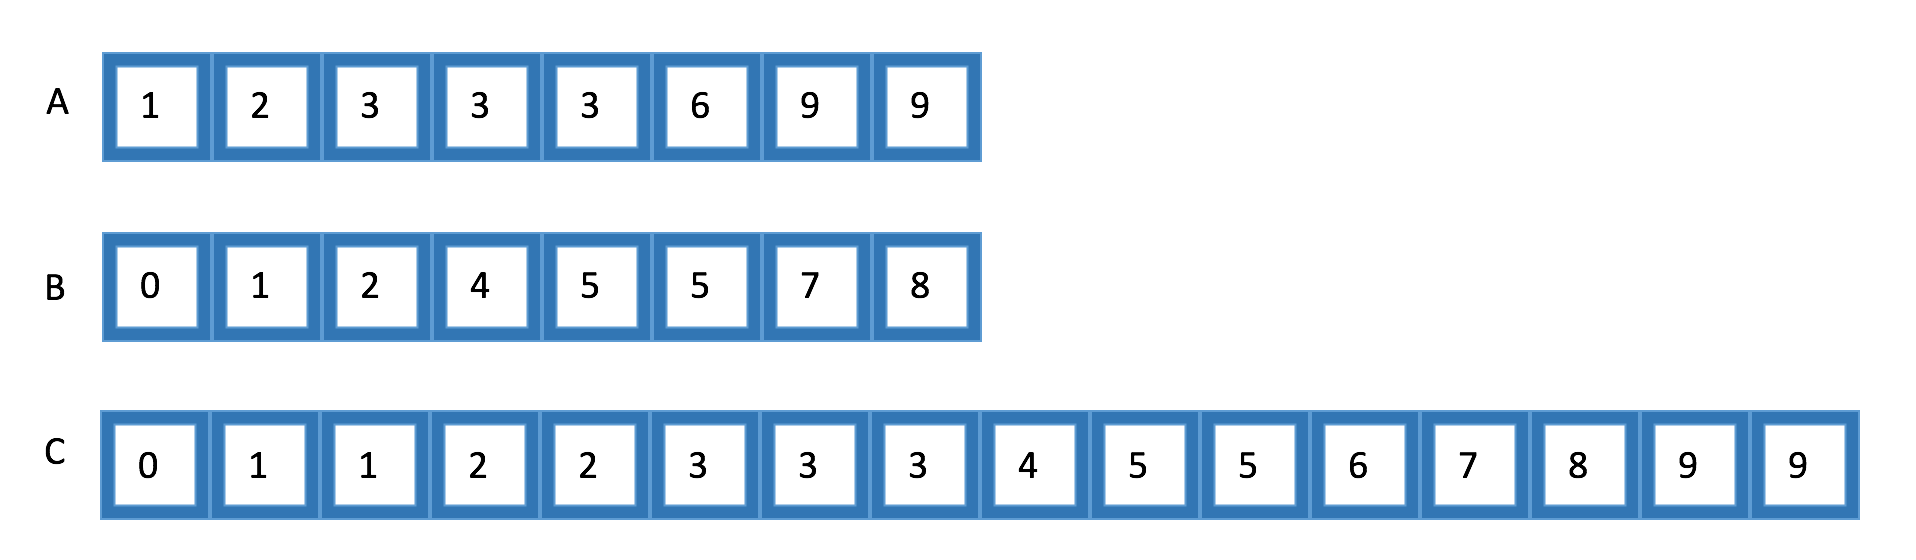
\includegraphics{merge.png}
}
\end{center}
\caption{{\label{fig:merge}} Merge Example}
\end{figure}

Sequentially merging two sorted arrays has been solved for a long time. Listing 
\ref{list:merge_origin} shows the sequential code implemented in C++.  
The time complexity of this implementation is $O(m+n)$. 

        \begin{minipage}{\linewidth}
        \begin{singlespace}
        \begin{lstlisting} [caption = {Sequential Merge Implementation in C++}, captionpos=b, label = {list:merge_origin}]
void merge(int *A, int m, int *B, int n, int *C) 
{
    int i, j, k, l;
    i = 0;              //index A
    j = 0;              //index B
    k = 0;              //index C
  
    /* handle the start of A[] and B[] */
    while ((i < m) && (j < n))
    {
        if (A[i] <= B[j]) {
            C[k] = A[i];
            i++;
        } else {
            C[k] = B[j];
            j++;
        }
        k++;
    }
    if (i == m) {       //handle remaining b[]
        for (l = j; l < n; l++) 
        {
            C[k] = B[l];
            k++;
        }
    } else {            //handle remaining a[]
        for (l = i; l <m; l++) 
        {
            C[k] = A[l];
            k++;
        }
    }
}
        \end{lstlisting}
        \end{singlespace}
        \end{minipage}


Merge is an important operation in contemporary computing systems. It is used as a subroutine
by many popular algorithms and applications such as merge sort 
and database operations. Therefore, the performance of merging is critical. 

As single-chip multiprocessors (CMPs) become more and more popular, parallel merging algorithms are 
developed to exploit the performance of CMPs. 
In \cite{pmalgo}, Siebert et al. proposed a parallel merge algorithm. 
With $p$ processing elements, 
the time complexity of merge could be reduced from $O(m+n)$ to $O(\frac{m+n}{p} + \log min(m,n))$.
This parallel merge algorithm can be implemented on CMPs using openMP with minimum effort, 
and achieve considerable speedup compared to
the sequential merge. 

However, a direct implementation of this parallel merge algorithm on GPU will result in 
suboptimal performance due to the architecture difference between GPU and CMP. To exploit the massive parallelism on GPU, we need to 
coordinate the memory access pattern, make full use of the shared memory and reduce the thread
divergence. This thesis proposes a novel GPU implementation for merging two sorted arrays. To the 
best of our knowledge, \textbf{thrust library} is the fastest GPU merge implementation. Our 
implementation achieves 5x speedup compared to the thrust library for certain input size.

The rest of the paper is organized as follows: 
Motivation for improving the performance of merge is presented in Chapter \ref{chap:motivation}.
GPU architecture and global memory coalescing are introduced in Chapter \ref{chap:architecture}.  
The parallel merge algorithm \cite{pmalgo} is described in Chapter \ref{chap:algo}. 
Chapter \ref{chap:implementation} describes the GPU implementation of the parallel merge algorithm
and all the optimizations. 
Evaluation is present in Chapter \ref{chap:evaluation}. 
Finally, Chapter \ref{chap:conclusion} concludes the thesis.
	% for INTRODUCTION in "introduction.tex"
\chapter{Motivation}\label{chap:motivation}
Merge is a very important operation. It is used as a subroutine by many popular algorithms and
applications such as merge sort and database operations. As a frequently used subroutine,
the performance of merging is critical. 

The time complexity of sequentially merging two sorted arrays is $O(m+n)$.
As the need for high performance computing grows, CMPs become more 
and more popular. However, most existing sequential algorithms cannot fully utilize the
computing resource on CMPs. To exploit the performance of CMPs, parallel algorithm must 
be developed. 

Siebert et al. \cite{pmalgo} proposed a parallel merge algorithm. With $p$ processing elements, 
the time complexity of merge could be 
reduced from $O(m+n)$ to $O(\frac{m+n}{p} + \log min(m,n))$ \cite{pmalgo}. This algorithm can be 
implemented on CMPs using openMP with minimum effort, and can achieve 
considerable speedup compared to sequential merge. 

Compared to CPU, GPU has more cores and larger memory bandwidth. For data parallel
applications, GPU has much better performance than CPU. 
Merge can also run on GPU. To the best of our knowledge, 
thrust library has the fastest GPU merge implementation. 
However, its throughput is still far from the memory bandwidth.


We implemented Siebert's parallel merge algorithm (we call it Naive Parallel Merge) and compared 
its performance to the thrust library. The memory throughput for different input
sizes is shown in figure \ref{fig:motivation}. 

\begin{figure}[!h]
\begin{center}
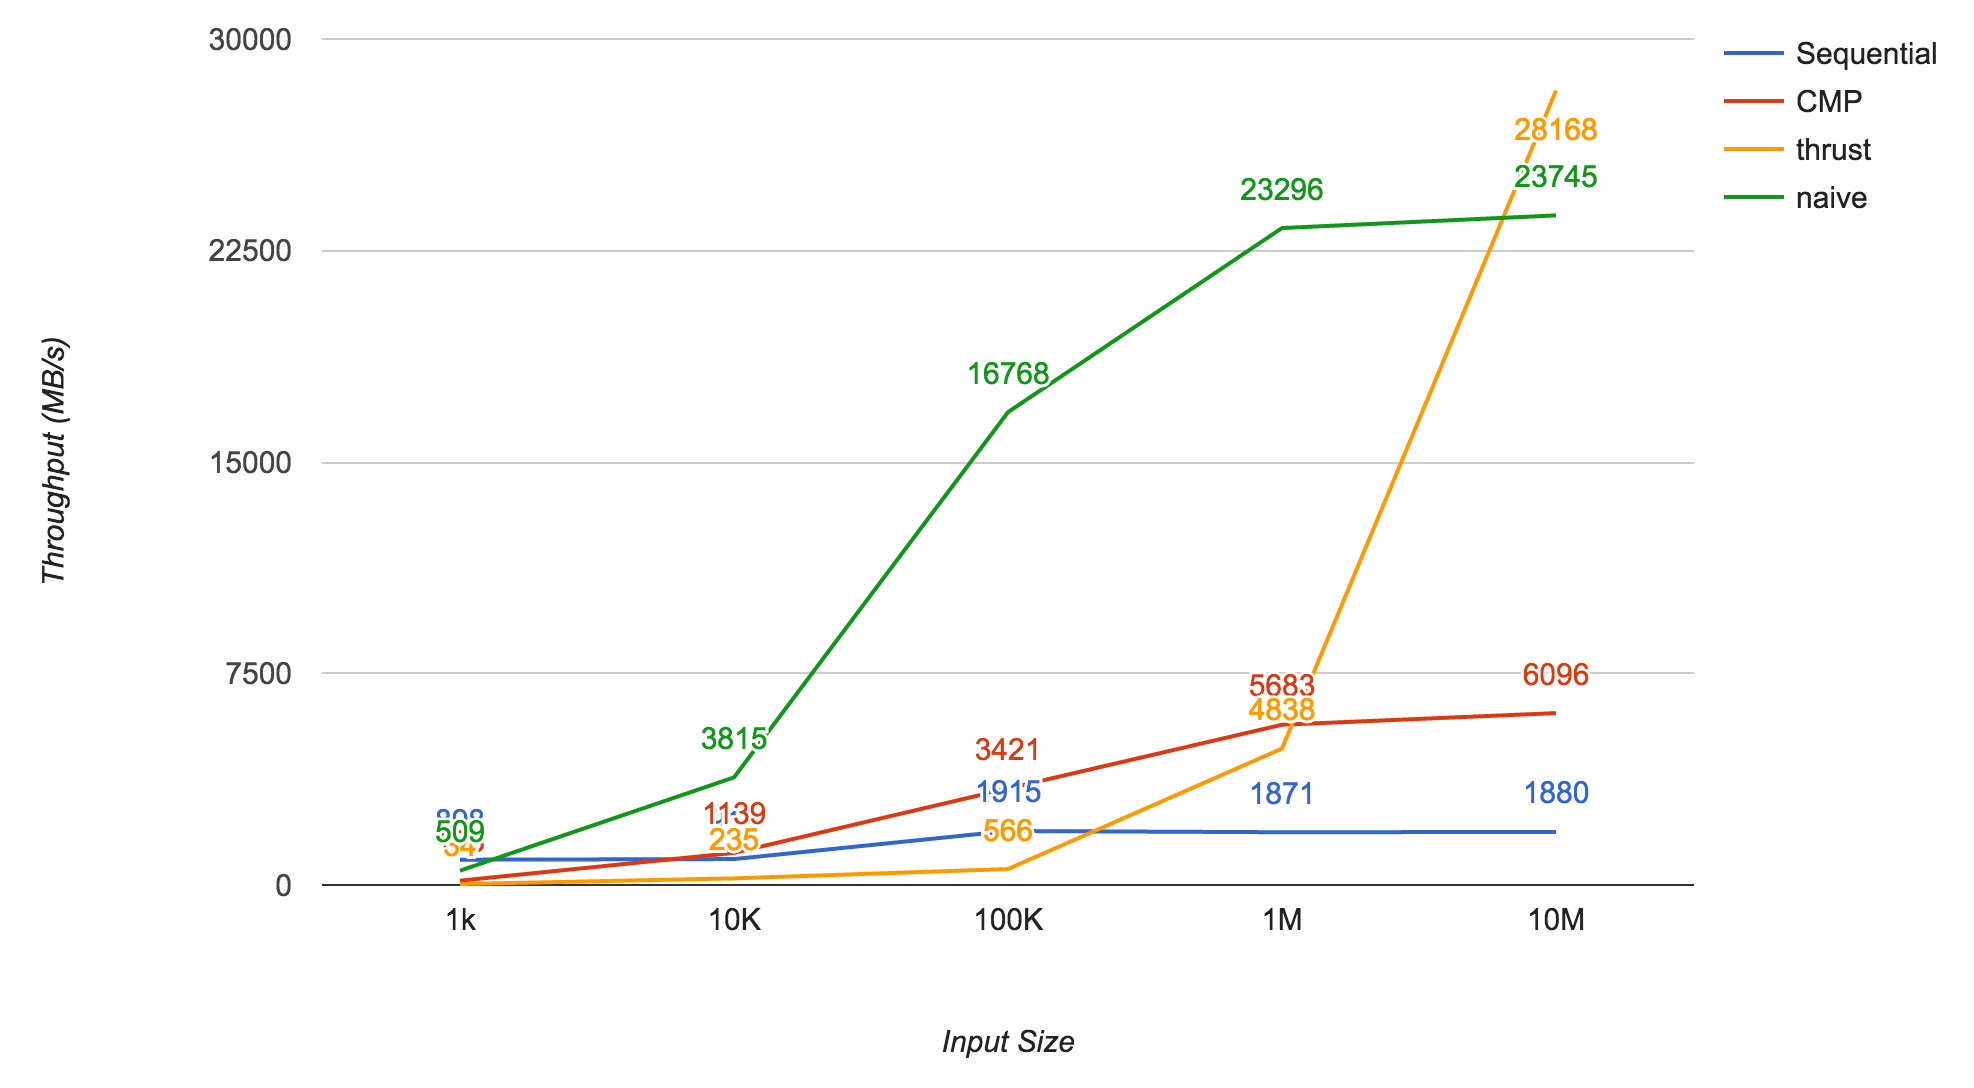
\includegraphics[width=\textwidth]{motivation.png}
\end{center}
\caption{{\label{fig:motivation}} Performance of Thrust Merge and Naive Parallel Merge on GTX980}
\end{figure}

Although naive parallel merge is suboptimal due to the lack of GPU-specific optimizations, 
we observe that for some input sizes (from 1k to 1M), its performance is better than 
that of thrust library.  

This motivates us to do further optimizations on naive parallel merge, and find a better 
GPU merge implementation that outperforms thrust library.  
\chapter{GPU Architecture and Global Memory Coalescing}\label{chap:architecture}

    \section{GPU Architecture}\label{sect:GPUArchitecure}
    \begin{itemize}
    \item   \textbf{Computation:} GPUs are designed for high computation throughput instead of 
            low latency. GPUs typically contain hundreds of cores. Programmers are allowed to
            set the number of blocks and the number of threads for each block to create massive
            parallelism that utilizes the huge number of cores on a GPU.
    \item   \textbf{Memory hierarchy:} The GPU memory hierarchy consists of global memory, shared memory 
            and registers. Global memory is shared across thread blocks. It is the largest 
            in terms of size. However, it is the slowest. Shared memory is shared only among 
            the threads in a single block. It is faster than global memory but slower than registers. 
            The size of shared memory is limited. In all the GPUs we use, the shared memory size per
            block is 48 KB. Registers are the fastest but have the smallest size.
    \end{itemize}

    \section{Baseline Architecture}\label{sect:baseline}
    The CPU and GPUs and their specifications are listed as follows:
\begin{itemize}
    \item CPU: Intel Core i7-4960HQ Processor, 2.6 GHz
    \item GPU: Nvidia Titan-Z, Kepler Architecture
    \item GPU: Nvidia GTX980, Maxwell Architecture
 \end{itemize} 
    

    \section{Global Memory Coalescing}\label{sect:coalesce}
    When we launch a kernel on GPU, it is executed by the parallel threads. 
    If the kernel has a global memory reference, then each thread will also generate a
    global memory request, and the memory addresses for each thread will most likely be 
    different. Listing \ref{list:coalesce} shows an example of global memory reference.

    \begin{minipage}{\linewidth}
    \begin{singlespace}
    \begin{lstlisting} [caption = {Memory Access Pattern}, captionpos=b, label = {list:coalesce}]
__global__ void kernel(int* a) 
{
    int tid = threadIdx.x;
    a[tid] = tid;
}
    \end{lstlisting}
    \end{singlespace}
    \end{minipage}

    These memory requests are grouped into a number of memory transactions. 
    When consecutive threads access consecutive global memory addresses 
    (as in Listing \ref{list:coalesce}), we call this coalesced access. 
    When coalesced access happens, a single transaction may be implemented \cite{cgo_arch} 
    to maximize the bandwidth usage.

    When the memory addresses accessed by threads are not consecutive 
    (e.g., for an access $a[tid * N]$ instead of $a[tid]$ in Listing \ref{list:coalesce}), 
    we call this non-coalesced access. 
    It is not possible anymore to pack the different requests from different threads 
    into a single transaction. In the worst case, we may need to make one transaction 
    per thread. This will result in a poor usage of memory bandwidth. 
    
    It is desirable to make all the accesses to global memory coalesced. One approach is to 
    use the shared memory as the scratch pad. This approach requires complex code 
    restructuring and is one of the GPU-specific optimizations that we use to improve the 
    performance of parallel merge. 


\chapter{Parallel Merging Algorithm}\label{chap:algo}

In \cite{pmalgo}, Siebert et al. proposed a parallel merge algorithm,
in which each processing element will calculate the output range it is
going to produce, and 
use that output range as the input to a \textbf{co-rank function} to identify the corresponding input
ranges that generate the output. Finally, each processing element will call the sequential merge
function to do the merge independently in parallel.

    \section{Co-rank Function}\label{sect:corank}
    Let $A$ and $B$ be two input arrays with $m$ and $n$ elements respectively. Both input arrays 
    are sorted 
    according to an ordering relation $\leq$. The index of the arrays starts from $0$. 
    The task is to merge $A$ and $B$ into an array $C$ with $m+n$ elements. 
    They use $C[m+n] = merge(A[m],B[n],\leq)$ to denote this task.
    In their paper, Siebert et al. pointed out two observations:
    \begin{itemize} 
        \item   For any $i$, $0 \leq i < m+n$ in $C$, there is either a $j$, $0 \leq j < m$ such that 
                $C[i] = A[j]$ or a $k$, $0 \leq k < n$ such that $C[i] = B[k]$. 
        \item   For any $i$-element prefix $C[0,...,i-1]$ of $C$, there must be indices $j$ 
                and $k$ of $A$ and $B$ such that $C[0,...,i-1] = merge(A[0,...,j-1],
                B[0,...,k-1],\leq)$.
    \end{itemize}
    Siebert et al. also proved that $j$ and $k$, which define
    the prefixes of $A$ and $B$ needed to produce the prefix of C of length $i$, are unique. 
    For an element $C[i]$, they call the index $i$ its rank. And they call the unique indices $j$ and $k$ 
    its co-ranks. Consequently, 
    they use the term \textbf{co-rank} for the process of determining $j$ and $k$ from $A, m, B, n$ and $i$.
    Notice that $i = j + k$ because the number of elements in the output array equals the sum of the number of elements
    in the input arrays. 
    Figure \ref{fig:corank} shows an example of co-rank. In this example, $C[16] = merge(A[8],B[8],\leq)$.
    $C[8] = merge(A[5],B[3],\leq)$. Therefore, the co-rank of $8$ is $5$ and $3$.  

    \begin{figure}[!h]
    \begin{center}
    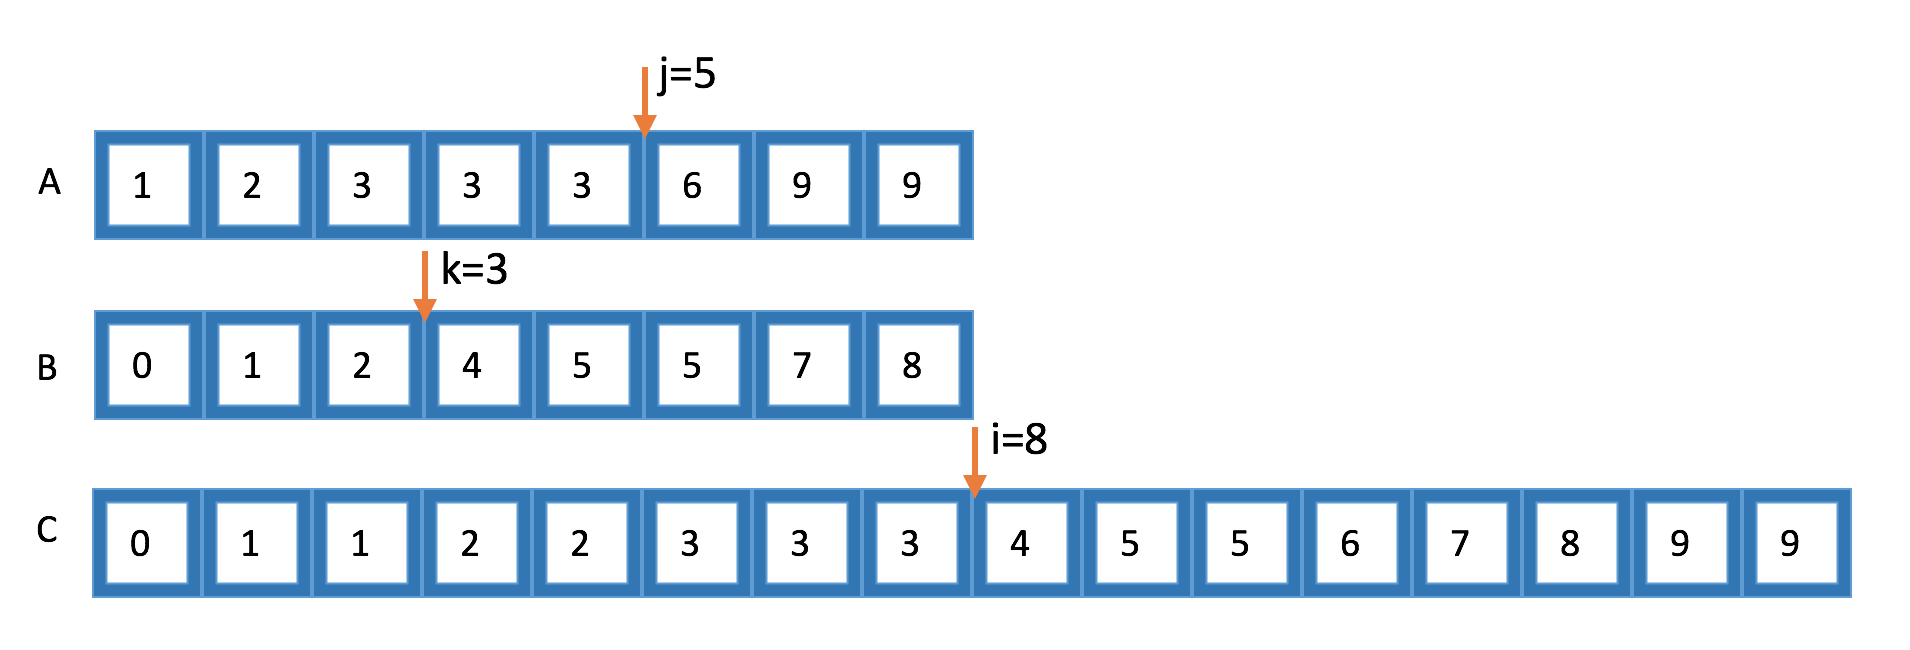
\includegraphics[width=\textwidth]{corank.png}
    \end{center}
    \caption{{\label{fig:corank}} Co-rank Example}
    \end{figure}

    The pseudo code to find the co-rank from $A, m, B, n$ and $i$ is also given in their paper.  
    In listing \ref{list:corank_origin}, we transform their pseudo code into the C++ implementation of 
    co-rank function. We calculate
    $j$ by using $j = co\_rank\_j(i, A, m, B, n)$. Then we calculate $k$ by $k = i - j$.  

    \begin{minipage}{\linewidth}
    \begin{singlespace}
    \begin{lstlisting} [caption = {Original Co-rank}, captionpos=b, label = {list:corank_origin}]
int co_rank_j(int i, int* A, int m, int* B, int n)
{
    int j = i < m ? i : m;                //j = min(i,m)
    int k = i - j;
    int j_low = 0 > (i-n) ? 0 : i-n;      //j_low = max(0, i-n) 
    int k_low;
    int delta;
    bool active = true;

    while(active)
    {
        if (j > 0 && k < n && A[j-1] > B[k]) {
            delta = ((j - j_low - 1) >> 1) + 1;
            k_low = k;
            j = j - delta;
            k = k + delta;
         } else if (k > 0 && j < m && B[k-1] >= A[j]) {
            delta = ((k - k_low - 1) >> 1) + 1;
            j_low = j;
            j = j + delta;
            k = k - delta;
        } else {
            active = false;
        }
    }
    return j;
}
    \end{lstlisting}
    \end{singlespace}
    \end{minipage}

    \section{Overall Parallel Merge}\label{sect:overall}
    The co-rank function provides a simple and efficient way to perform merging in 
    parallel. Let $p$ processing elements be given, all of which can access input and 
    output arrays $A$, $B$ and $C$. Each processing element has its own id $r$, $0 \leq r < p$. 
    
    Each processing element will calculate the output range ($C[i\_start,...i\_end]$) it is 
    going to produce.  
    The output ranges can be chosen such that  
    they cover the whole output array of size $m + n$, and the size of output each processing
    element producing differs by at most $1$. 
    Then, each processing element computes the corresponding co-ranks for both the 
    start and end index. 
    These co-ranks determine the input ranges of the input arrays this processing element needs 
    to merge sequentially.  

    Listing \ref{list:pseudo_merge} shows the pseudo code for the parallel merge algorithm.

    \begin{minipage}{\linewidth}
    \begin{singlespace}
    \begin{lstlisting} [caption = {Pseudo Code for Parallel Merge Algorithm}, captionpos=b, label = {list:pseudo_merge}, mathescape=true]
void paralle_merge(int *A, int m, int *B, int n, int*C) 
{
    r       = processing_id;        // 0 <= r < p
    i_start = floor(r*(m+n)/p);     // start index of output 
    i_end   = floor((r+1)*(m+n)/p); // end   index of output 
    j_start = co_rank_j(i_strat, A, m, B, n);
    j_end   = co_rank_j(i_end,   A, m, B, n);
    k_start = i_start - j_start;
    k_end   = i_end   - j_end;
    merge( A[j_start,...,j_end-1], B[k_start,...,k_end-1],
           C[i_start,...,i_end-1] );
}
    \end{lstlisting}
    \end{singlespace}
    \end{minipage}

    Figure \ref{fig:overall} shows an example of the parallel merge process. In this example,
    there are two processing elements($p=2$). These two processing elements are going to do 
    the task $C[16] = merge(A[8],B[8],\leq)$ collaboratively in parallel. 

    \begin{figure}[!h]
    \begin{center}
    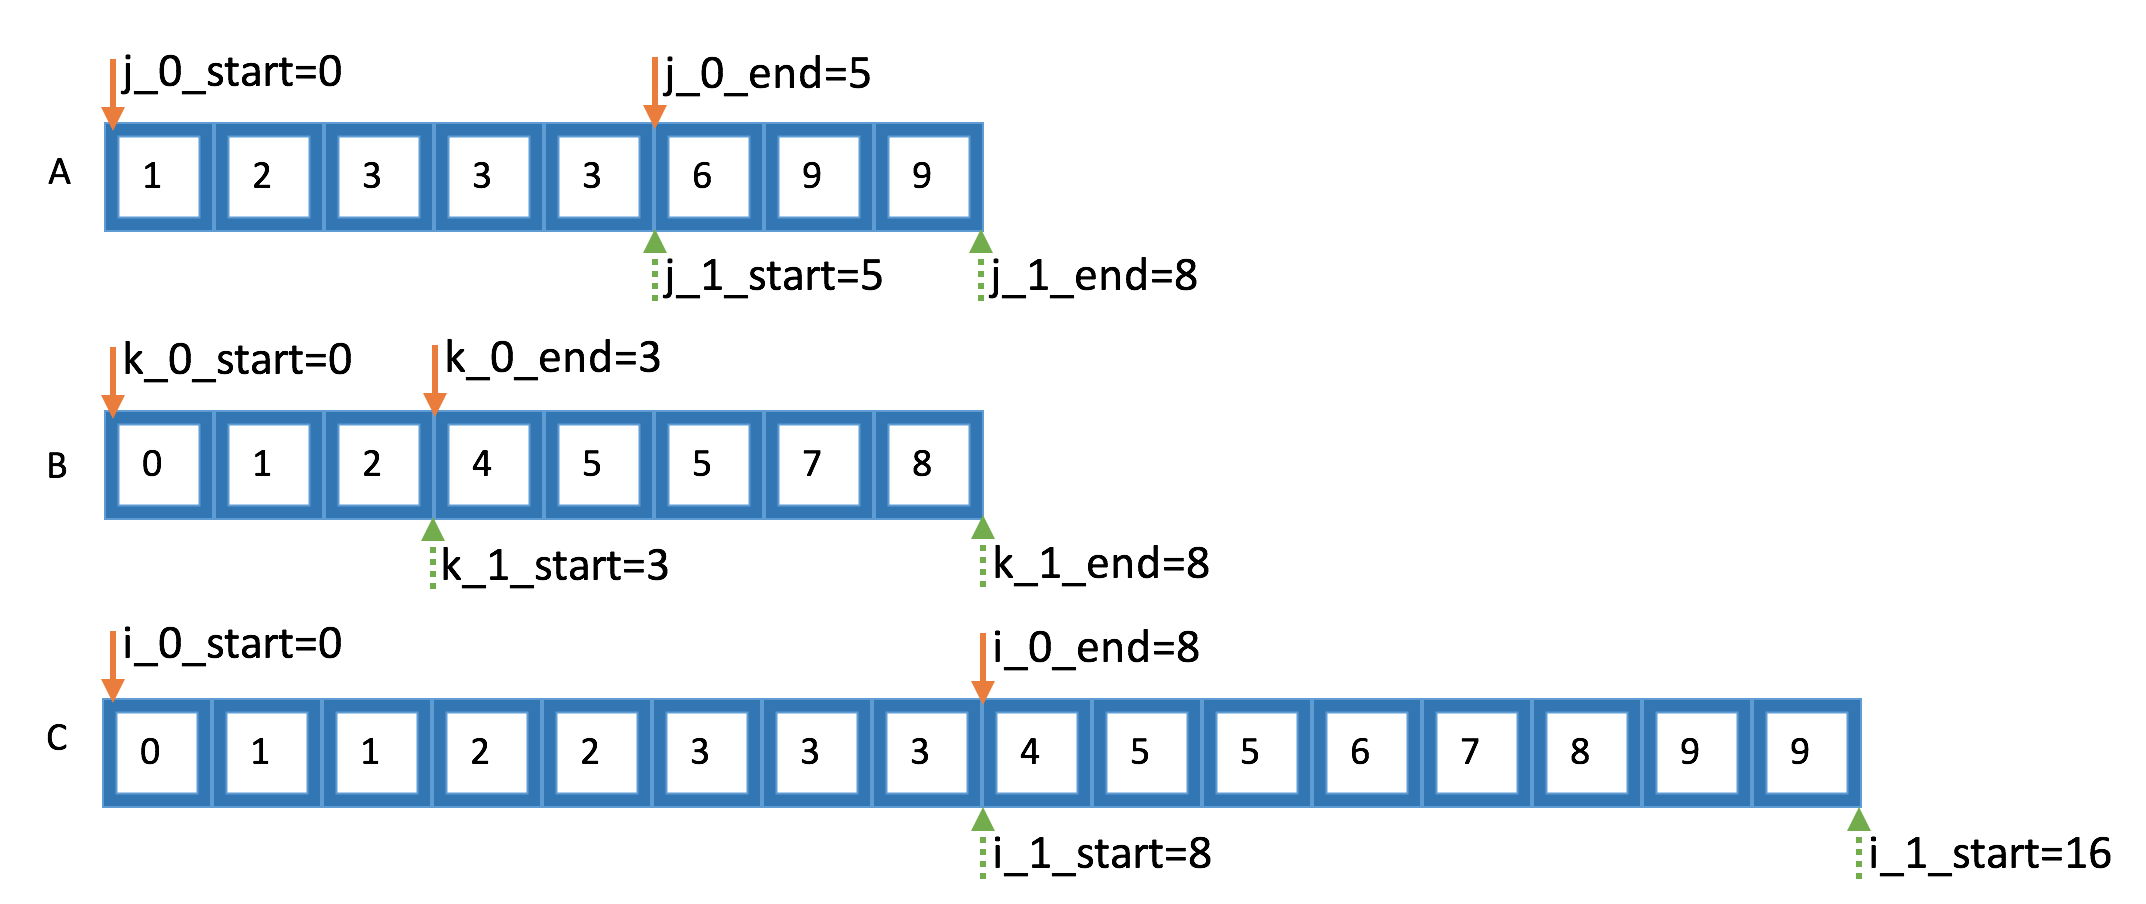
\includegraphics[width=\textwidth]{overall.png}
    \end{center}
    \caption{{\label{fig:overall}} Parallel Merge Algorithm Example}
    \end{figure}   
 
    For $p_0$ (solid red arrows), $r = 0$, $i\_start = 0$, $i\_end=8$. It is going to produce
    $C[0,...,7]$. After running the co-rank function, $p_0$ knows the input ranges: $j\_start = 0$, 
    $j\_end=5$, $k\_start = 0$, $k\_end=3$. Therefore, $p_0$ will call 
    $C[0,...,7] = merge(A[0,...,4],B[0,...,2],\leq)$.

    For $p_1$ (dashed green arrows), $r = 1$, $i\_start = 8$, $i\_end=16$. It is going to produce
    $C[8,...,15]$. After running the co-rank function, $p_1$ knows: $j\_start = 5$, 
    $j\_end=8$, $k\_start = 3$, $k\_end=8$. So $p_1$ will call 
    $C[8,...,15] = merge( A[5,...,7],B[3,...,7],\leq)$.

    Because $p_0$ and $p_1$ are working on different parts of the input and output, they can run in 
    parallel without interference. Also, the sizes of output they produce are the same. 
    Therefore, load balance is guaranteed.      



    % \section{Stable Merge}\label{sect:stable}
    % This subsection will discuss the property of stable merge.

    \section{Implementation on CPU}\label{sect:CPU}
    We implement the parallel merge algorithm on CMPs using openMP. 
    The CPU we are using has 8 threads. Each thread first calculates the output 
    range it is going to produce. Then it identifies the corresponding input ranges 
    using the co-rank function. 
    Finally, it does the merge in parallel by calling the sequential merge. 
    Ideally, the speedup of an 8 thread CPU could achieve 8. 
    In reality, the parallel merge is slower than sequential merge when the input size 
    is small. As the input size grows, parallel merge becomes faster, and can achieve a 
    speedup of 5x compared to the sequential merge.  
    
    For the small input size, parallel merge is slower than sequential merge because the 
    overhead of binary search from co-rank function dominates the actual merge. 
    As the input size grows, the overhead of binary search from co-rank could be amortized,
    and parallel merge could outperform the sequential merge. 
    However, the overhead of binary search cannot be neglected. 
    Moreover, memory congestion may occur because 
    the threads are issuing more memory requests when doing merge in parallel. Due to the
    non-negligible overhead and potential memory congestion, the actual speedup can achieve
    5x instead of 8. 
    Figure \ref{fig:CMP} shows the performance of CMP parallel merge over sequential merge.  

    \begin{figure}[!th]
    \begin{center}
    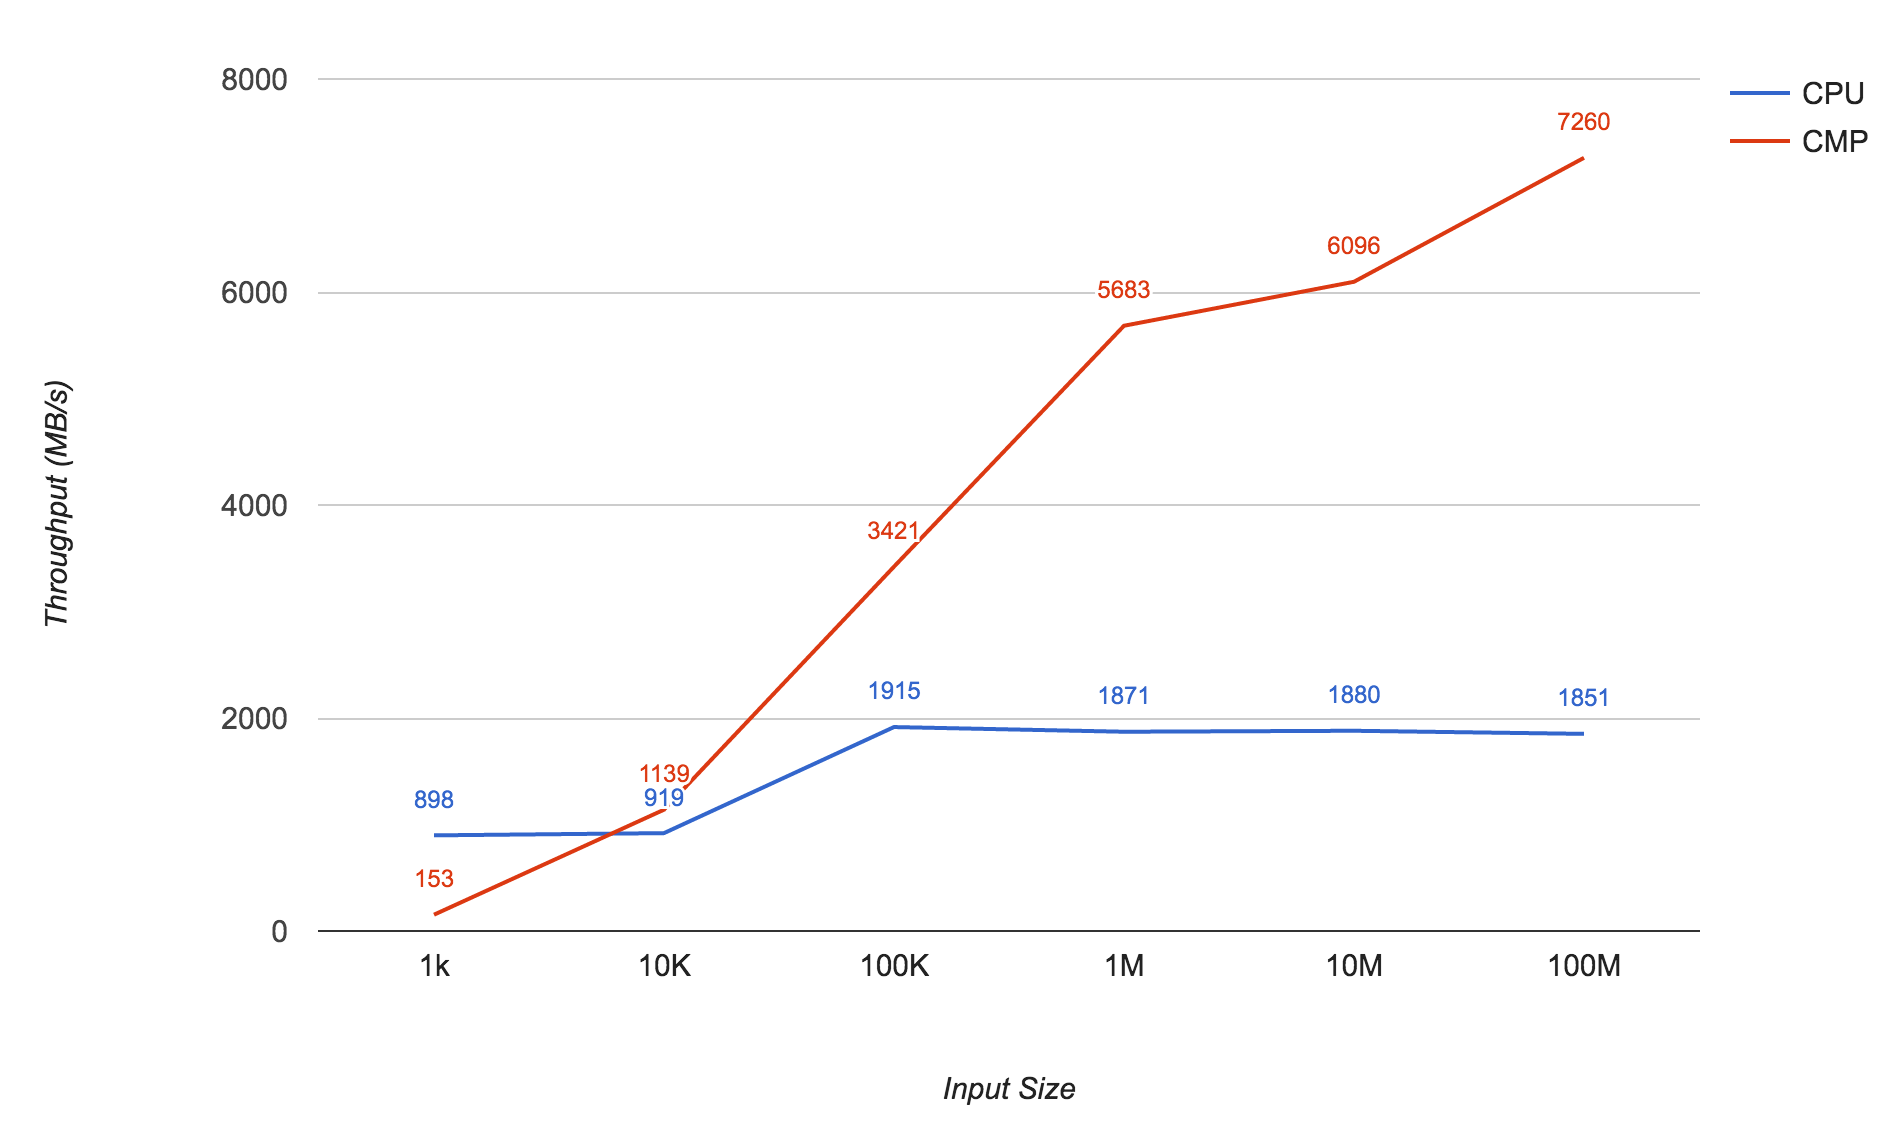
\includegraphics[width=\textwidth]{CMP.png}
    \end{center}
    \caption{{\label{fig:CMP}} CMP Merge and Sequential Merge}
    \end{figure}



\chapter{Parallel Merging Algorithm Implementation on GPU}\label{chap:implementation}
Compared to CMPs, GPUs have more threads and larger memory bandwidth 
for the purpose of massive parallelism. 
However, a direct translation of a parallel algorithm suits CMPs
may not run efficiently on GPUs. 
To explore massive parallelism on GPUs, we need to coordinate 
the memory access pattern, make full use of the shared memory, reduce the thread 
divergence, improve the load balance for different processing units, and create enough 
parallelism.

As the first step, we implement this parallel merge algorithm on GPU without any 
GPU-specific optimization. We 
name it \textbf{naive parallel merge}. More details about naive parallel merge 
are described in section \ref{sect:naive}. 

However, the naive parallel merge did not incorporate any GPU-specific optimizations, 
which is critical to improve the application performance that runs on GPU.  
We implement an optimized GPU version that utilizes shared memory as a scratch pad to make the 
accesses to global memory coalesced. We name it \textbf{single buffer 
parallel merge}. More details about single buffer parallel merge are described in section 
\ref{sect:single}. 

In single buffer parallel merge, we only consume half of the 
data we load into the shared memory. The other half is wasted. 
To better utilize the data we load into shared memory, we implement a third version. And we 
name it \textbf{double buffer parallel merge}. We describe more details about double buffer 
parallel merge in section \ref{sect:double}.

%%%%%%%%%%%%%%%%%%%%%%%%%%%%%%%%%%%%%%%%%%%%%%%%%%%%%%%%%%%%%%%%
%   
%   Naive Parallel Merge
%
    \section{Naive Parallel Merge}\label{sect:naive}
    In naive parallel merge, we copy the input arrays $A[\,]$ and $B[\,]$ from host to device global 
    memory first.
    Then each thread calculates the thread index ($r$) and total number of threads ($p$) 
    using $t\_id = blockIdx.x * blockDim.x + threadIdx.x$ and $t\_num = gridDim.x * blockDim.x$ 
    respectively. Based on $t\_id$ and $t\_num$, each thread calculates the output range it is 
    going to produce, and uses the output range as the input to the co-rank function to identify the 
    corresponding input ranges. After getting the input ranges, all threads can start to merge 
    independently by calling the sequential merge function in parallel and writing the result
    to $C[\,]$ in device global memory. Finally, we copy $C[\,]$ from device global memory back to the host.

    Figure \ref{fig:naive} shows an example of naive parallel merge. $A[\,]$, $B[\,]$ and $C[\,]$ 
    are in device global memory. This example shows the work of one thread. After identifying
    its output range($C[\,]$) and input ranges($A[\,]$, $B[\,]$), it uses sequential merge to write the
    result to $C[\,]$. All the threads will run in parallel and produce the result for the entire 
    output array $C[\,]$.   

    \begin{figure}[!h]
    \begin{center}
    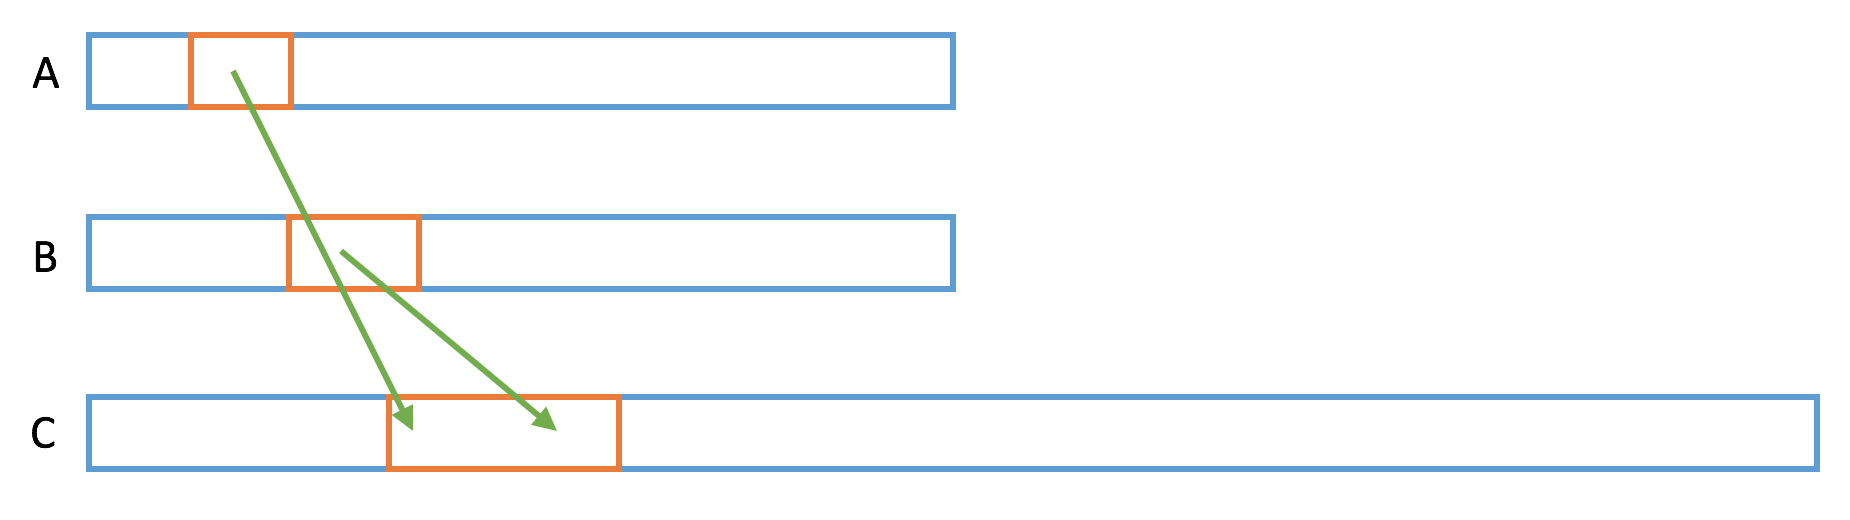
\includegraphics[width=\textwidth]{naive.png}
    \end{center}
    \caption{{\label{fig:naive}} Naive Parallel Merge}
    \end{figure}

    The performance of naive parallel merge on titan-z is shown in Figure \ref{fig:naive_evaluation}.
      
    \begin{figure}[!h]
    \begin{center}
    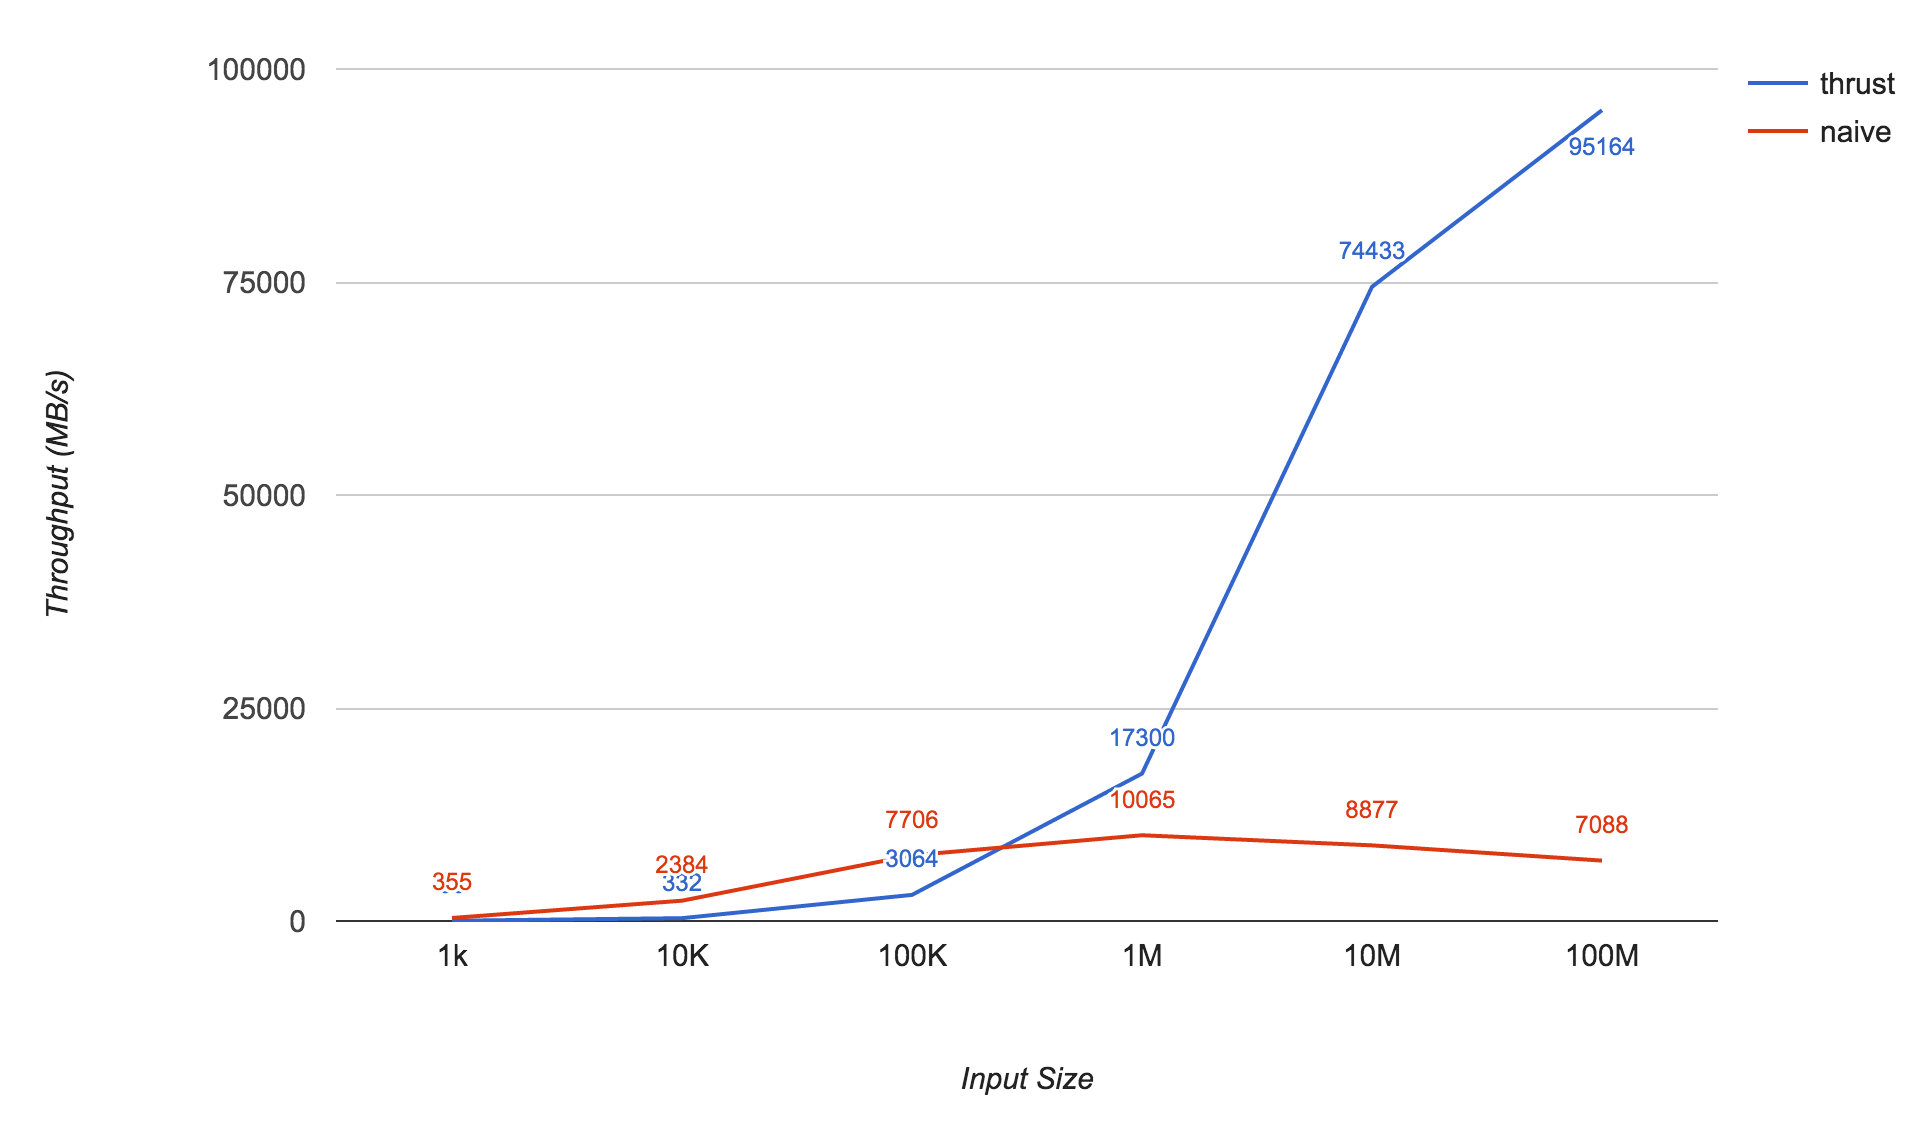
\includegraphics[width=\textwidth]{naive_evaluation.png}
    \end{center}
    \caption{{\label{fig:naive_evaluation}} Performance of Naive Parallel Merge on Titan-Z}
    \end{figure}

    In naive parallel merge, both the co-rank function and merge function run on the global memory. Due to 
    the nature of the co-rank function, in which each thread is doing a binary search for its own input 
    index, the memory access pattern is not coalesced. The memory access pattern for merger function
    is not coalesced either. For these reasons, although naive parallel merge is faster than thrust merge 
    for certain input size, it still underutilizes the memory 
    bandwidth offered by GPU and therefore did not achieve the optimal overall performance.


%%%%%%%%%%%%%%%%%%%%%%%%%%%%%%%%%%%%%%%%%%%%%%%%%%%%%%%%%%%%%%%%
%   
%   Single Buffer Parallel Merge
%
    \section{Single Buffer Parallel Merge}\label{sect:single}
    The memory access pattern in naive parallel merge is not coalesced. To improve the memory 
    throughput on GPU, coalesced global memory accesses pattern are critical. For this reason, 
    we use shared memory on GPU to make the access pattern to global memory coalesced in single
    buffer parallel merge. Single buffer parallel merge works as follows: Co-rank function is
    run in two levels, block level and thread level. In the block level, all the threads in 
    the same block do the same searching. Each thread calculates the block index and total 
    number of blocks using $b\_id = blockIdx.x$ and $b\_num = gridDim.x$ respectively. 
    Based on $b\_id$ and $b\_num$, all threads within the same block calculate the output range 
    that block is going to produce, and use the output range as the input to the co-rank function 
    to identify the corresponding input ranges for that block. The co-rank function is run on 
    global memory in the block level.  
    After knowing the input ranges for the block, all threads in the block cooperatively load the 
    input to the shared memory. In this way, we can guarantee that the global memory access 
    pattern is coalesced. 

    However, the shared memory may not be large enough to hold all the input data. 
    So we create a loop. In each iteration, we load $x$ elements from input array A and 
    $x$ elements from input array B into the shared memory. This will produce $x$ (not $2x$) 
    elements to the output array C. Because in extreme cases, all the output may come from 
    one of the input array, we waste half of the data loaded into the shared memory.
 
    Then we run the co-rank function in thread level. Threads in a block will merge $x$ 
    elements using the data we load into shared memory. So the co-rank function is run on 
    shared memory in the thread level.
    Each thread calculates the thread index and total number of threads in the block
    using $t\_id = threadIdx.x$ and $r\_num = blockDim.x$ respectively. 
    Based on $t\_id$ and $t\_num$, each thread calculates the output range 
    that thread is going to produce, and uses the output range as the input to the co-rank function 
    to identify the corresponding input ranges.  
    Then each thread can start its work independently and call the sequential merge function to do 
    the merge in parallel on the input we load to shared memory and write the output to device 
    global memory. Figure \ref{fig:single1} shows the first iteration of single buffer
    parallel merge. The solid orange box is the block level run of the co-rank function. The 
    dashed green box is the first iteration of the thread level run of co-rank function. 
    The data marked by the solid blue arrow are wasted.  

    \begin{figure}[!h]
    \begin{center}
    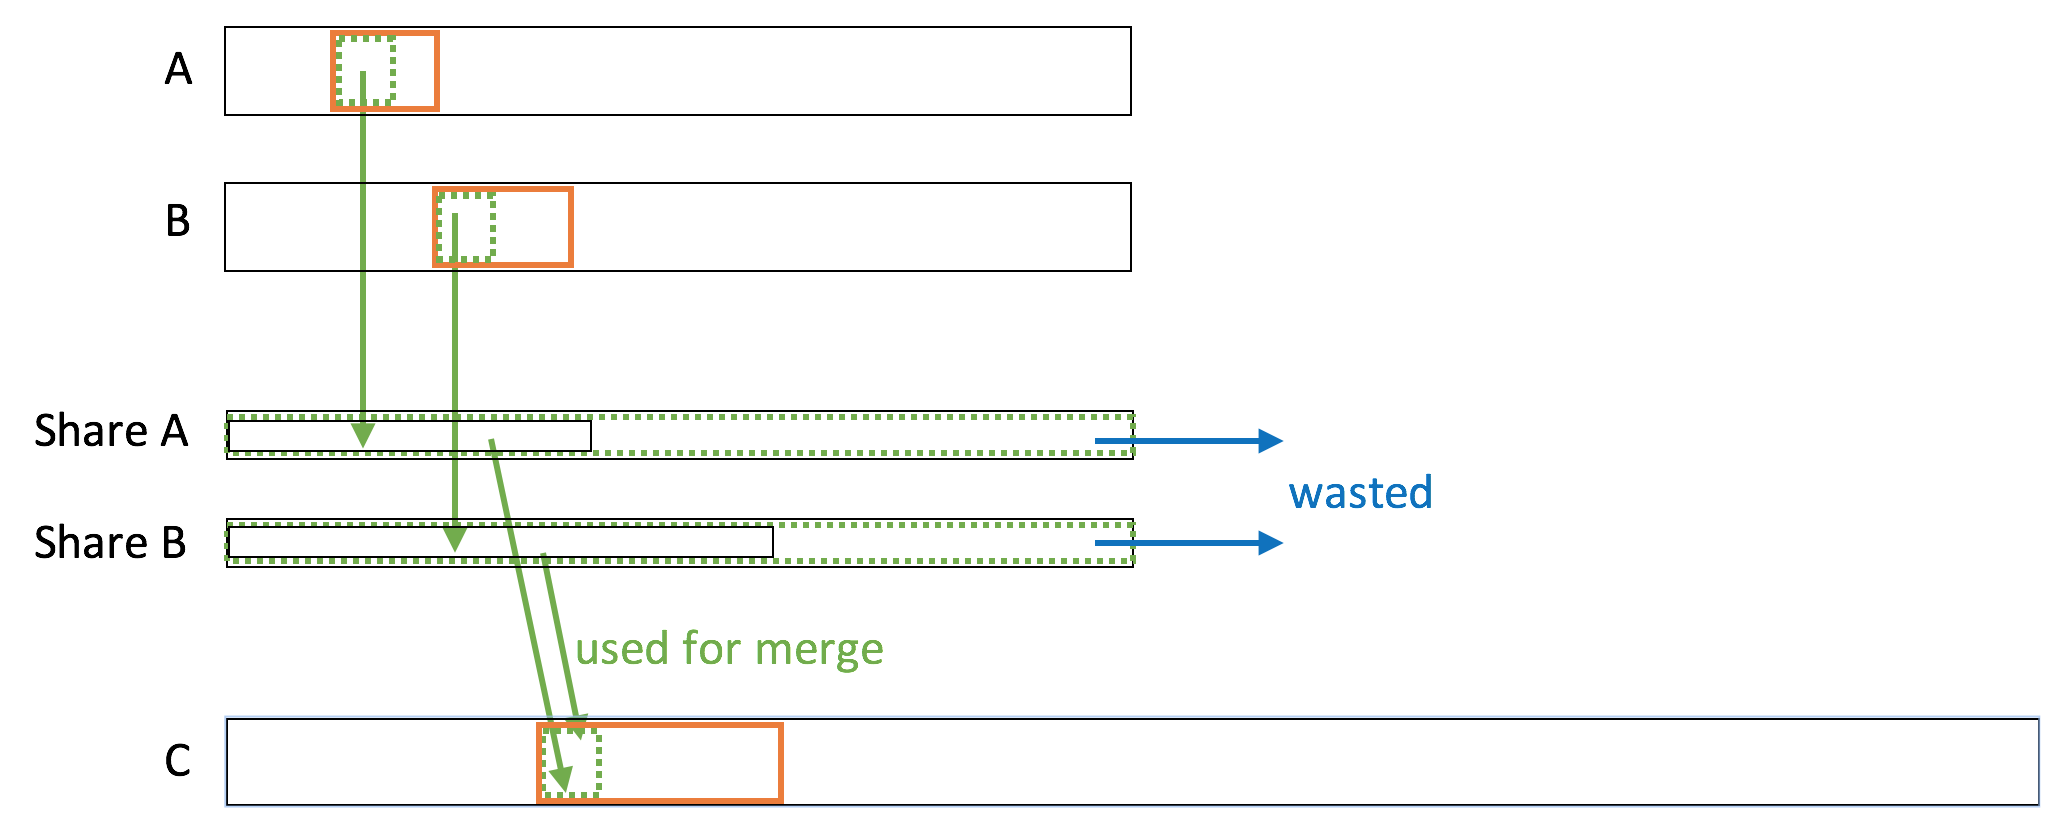
\includegraphics[width=\textwidth]{single1.png}
    \end{center}
    \caption{{\label{fig:single1}} First Iteration of Single Buffer Parallel Merge}
    \end{figure}

    In the next iteration, we will load the data we have not merged  
    into the shared memory, and do the same merge. 
    Figure \ref{fig:single2} shows the second iteration of single buffer
    parallel merge. The dashed red box is the second iteration of the thread level 
    run of co-rank function. 

    \begin{figure}[!h]
    \begin{center}
    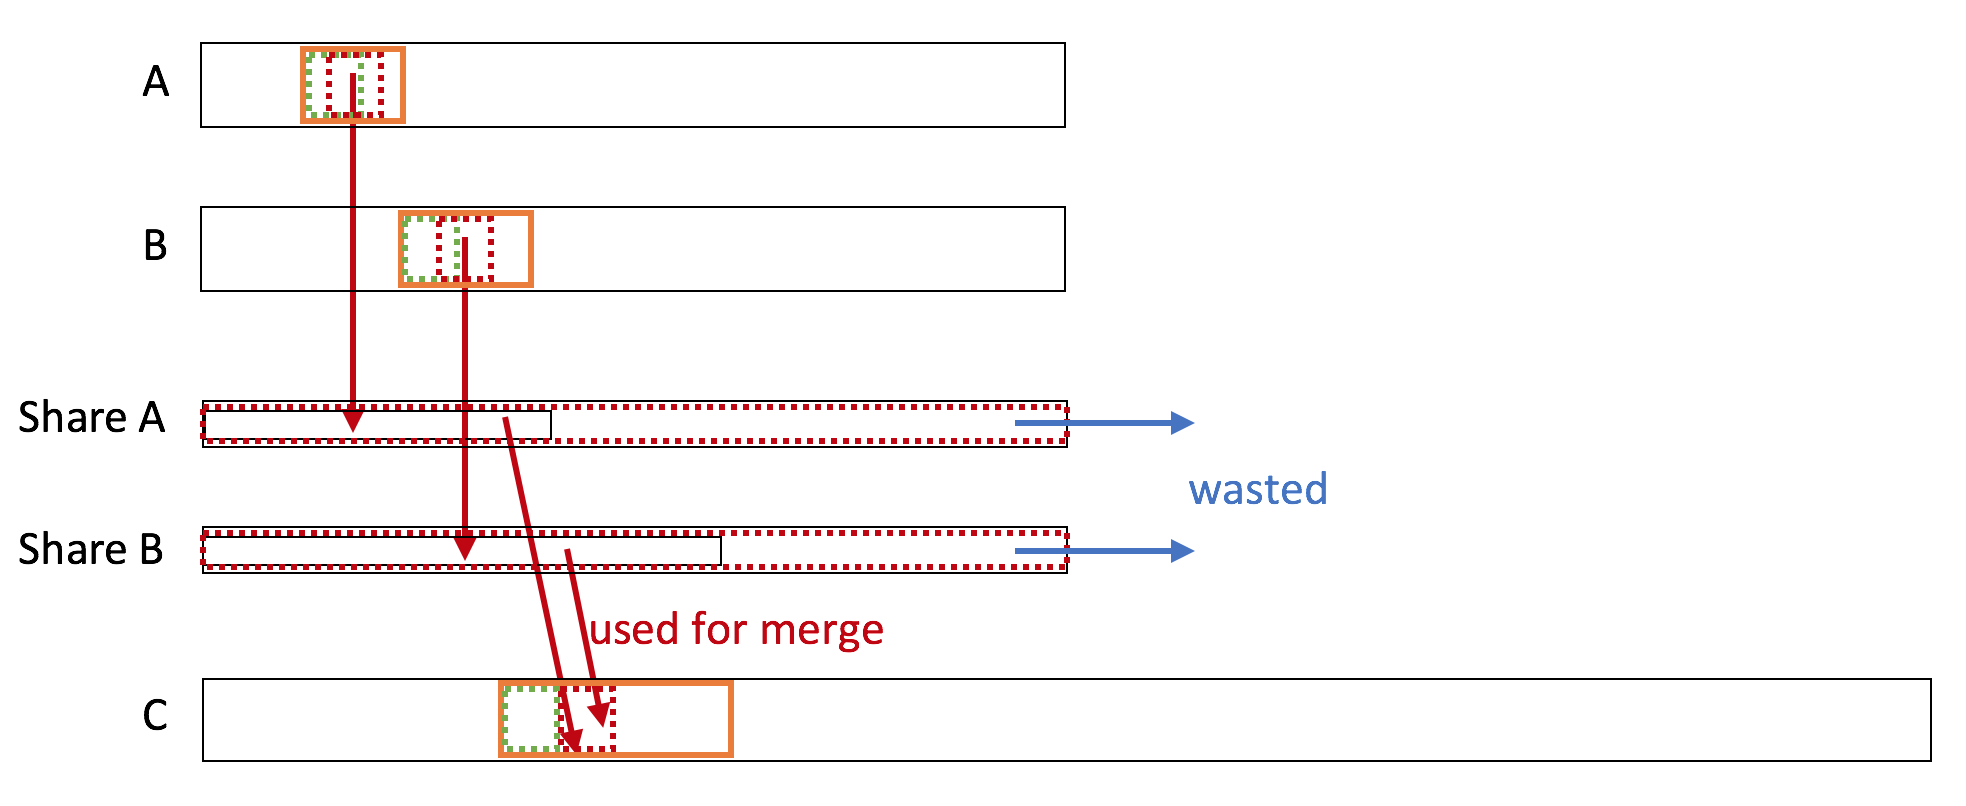
\includegraphics[width=\textwidth]{single2.png}
    \end{center}
    \caption{{\label{fig:single2}} Second Iteration of Single Buffer Parallel Merge}
    \end{figure}

    The loop runs until we have merged all the data that block is going to produce (filling 
    the entire solid orange box).   

    In single buffer parallel merge, we fill the shared memory in a coalesced pattern so that
    there will be fewer global memory requests. The thread level co-rank function runs on
    shared memory. The merge function reads the input from shared 
    memory, and writes to global memory. Because we convert many expensive global memory 
    reads to cheap shared memory
    reads, the single buffer parallel merge could better utilize the memory bandwidth and hence 
    outperform the naive parallel merge by 5x. 

    The performance of single buffer parallel merge is evaluated in Figure \ref{fig:single_evaluation}.

    \begin{figure}[!h]
    \begin{center}
    \resizebox{\textwidth}{!}{
        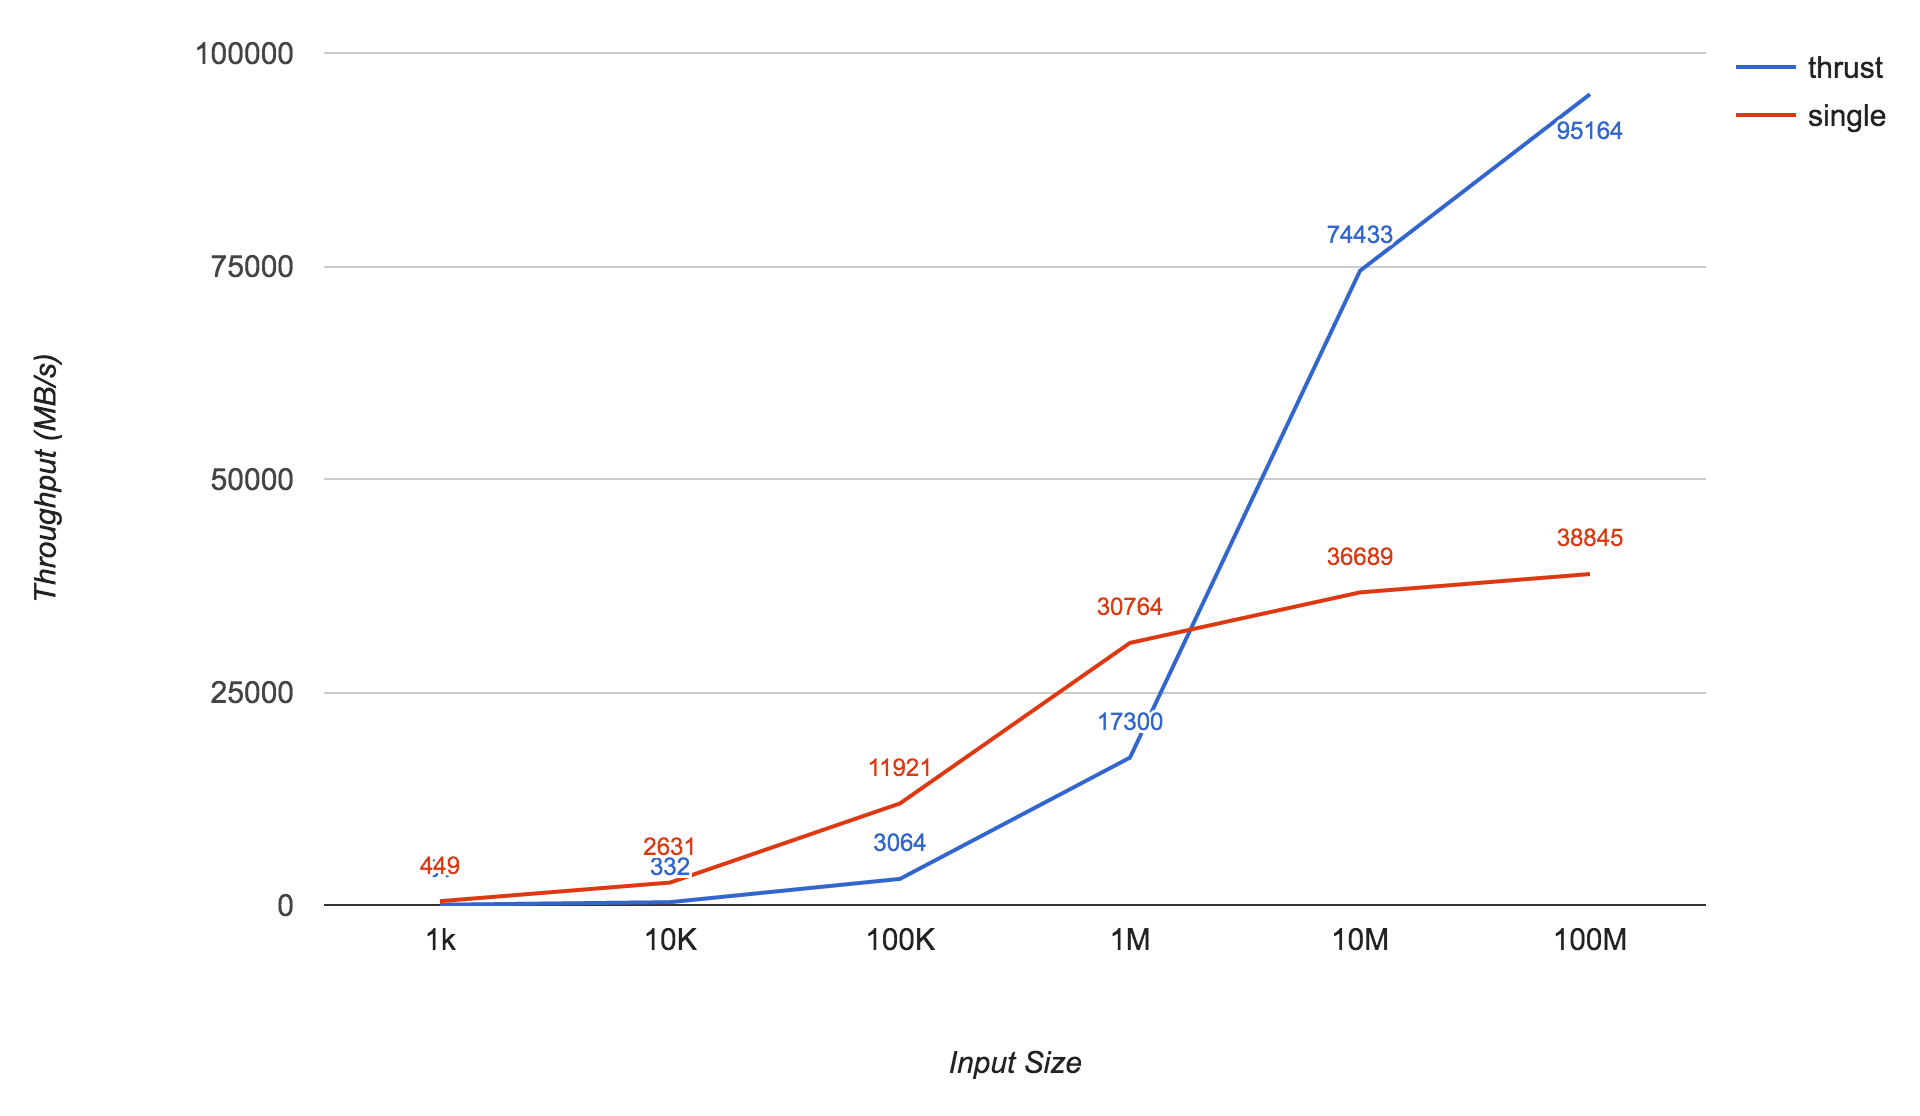
\includegraphics{single_evaluation.png}
    }
    \end{center}
    \caption{{\label{fig:single_evaluation}} Performance of Single Buffer Parallel Merge on Titan-Z}
    \end{figure}

%%%%%%%%%%%%%%%%%%%%%%%%%%%%%%%%%%%%%%%%%%%%%%%%%%%%%%%%%%%%%%%%
%   
%   Double Buffer Parallel Merge
%
    \section{Double Buffer Parallel Merge}\label{sect:double}
    In single buffer parallel merge, we only consume a half of the data we load into the shared 
    memory. The other half is wasted. To further 
    optimize the performance, we create the double buffer parallel merge, in which we 
    utilize all the data we load into the shared memory.

    The overall process is similar to single buffer parallel merge except for how we use
    shared memory. Co-rank function is
    run in two levels, block level and thread level. In the block level, all the threads in 
    the same block do the same searching. Each thread calculates the block index and total 
    number of blocks using $b\_id = blockIdx.x$ and $b\_num = gridDim.x$ respectively. 
    Based on $b\_id$ and $b\_num$, all threads within the same block calculate the output range 
    that block is going to produce, and use the output range as the input to the co-rank function 
    to identify the corresponding input ranges for that block. 
    After knowing the input ranges for the block, all threads in the block cooperatively load the 
    input to the shared memory.

    \begin{figure}[!h]
    \begin{center}
    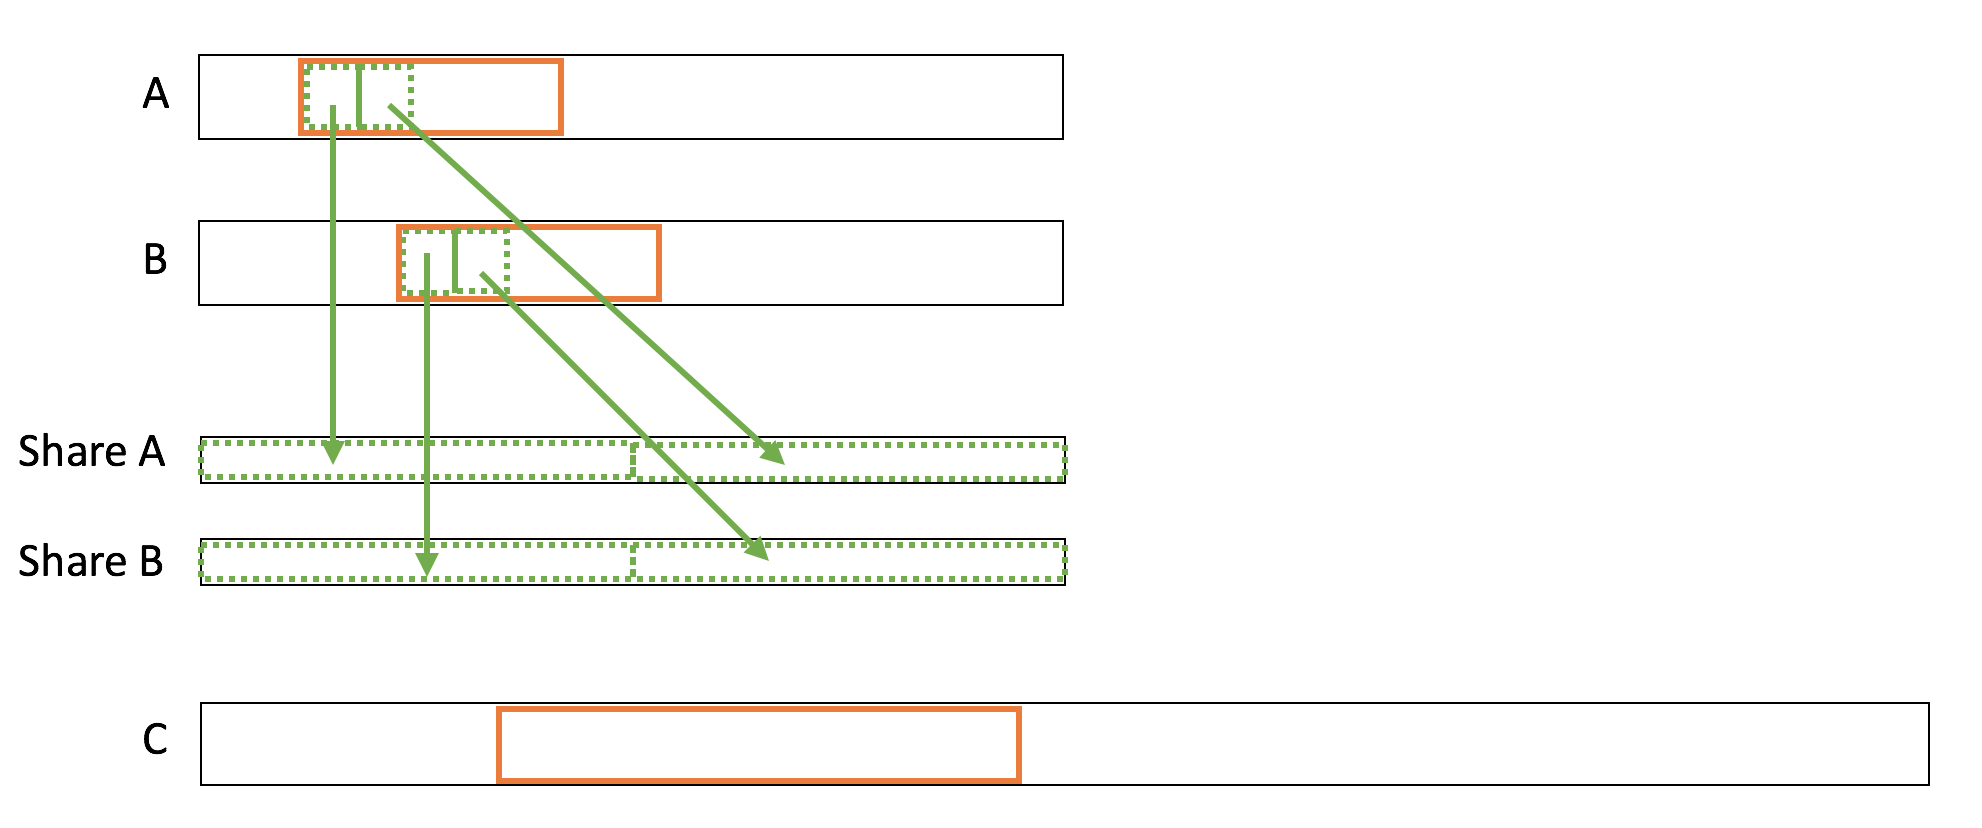
\includegraphics[width=\textwidth]{double0.png}
    \end{center}
    \caption{{\label{fig:double0}} Initialization of Double Buffer Parallel Merge}
    \end{figure}    

    We use a loop because shared memory may not be large enough to hold all the input data.
    When initializing, we load $2x$ elements from input array A and $2x$ elements from input 
    array B into the shared memory. Figure \ref{fig:double0} shows the initialization process.

    In each later iteration, all the threads in a block will produce $x$
    elements to the output array C. If there are more than $x$ elements in shared array A and 
    shared array B, we do not load from global memory. Figures \ref{fig:double1} and \ref{fig:double2} 
    show examples of the first iteration and second iteration of double buffer parallel 
    merge. In these two iterations, there are enough data remaining in the shared memory, 
    so we did not load from the global memory to shared memory.

    \begin{figure}[!h]
    \begin{center}
    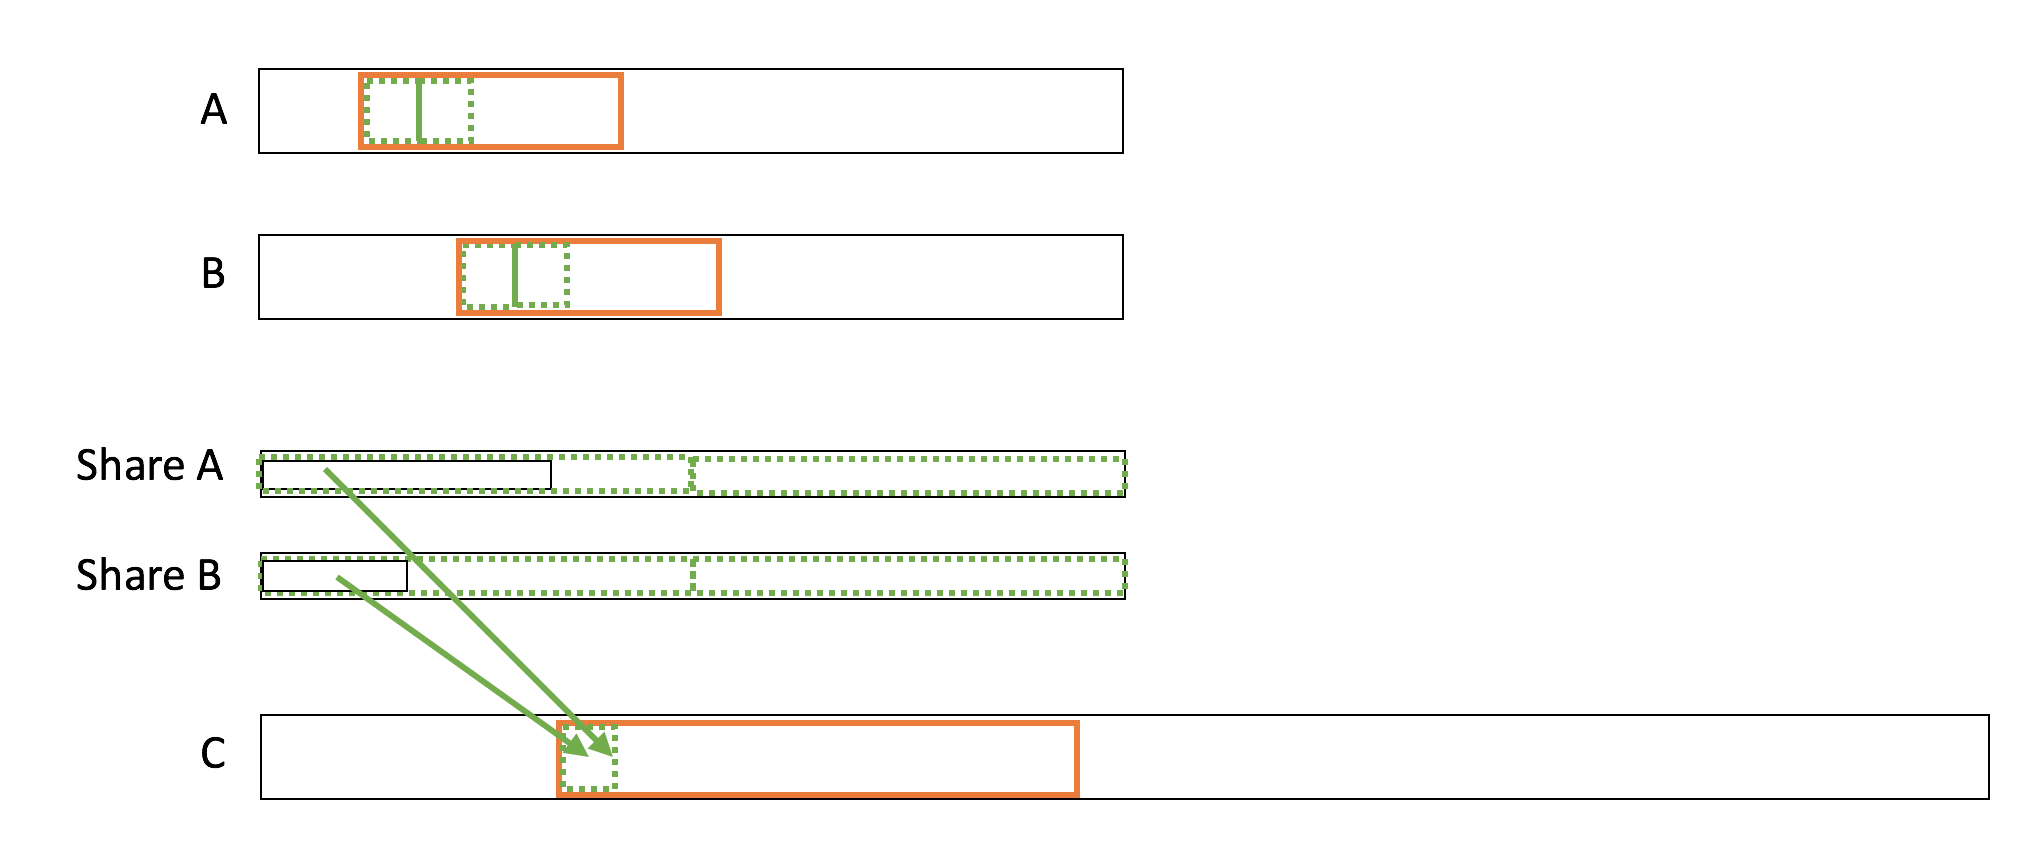
\includegraphics[width=\textwidth]{double1.png}
    \end{center}
    \caption{{\label{fig:double1}} First Iteration of Double Buffer Parallel Merge}
    \end{figure}

    \begin{figure}[!h]
    \begin{center}
    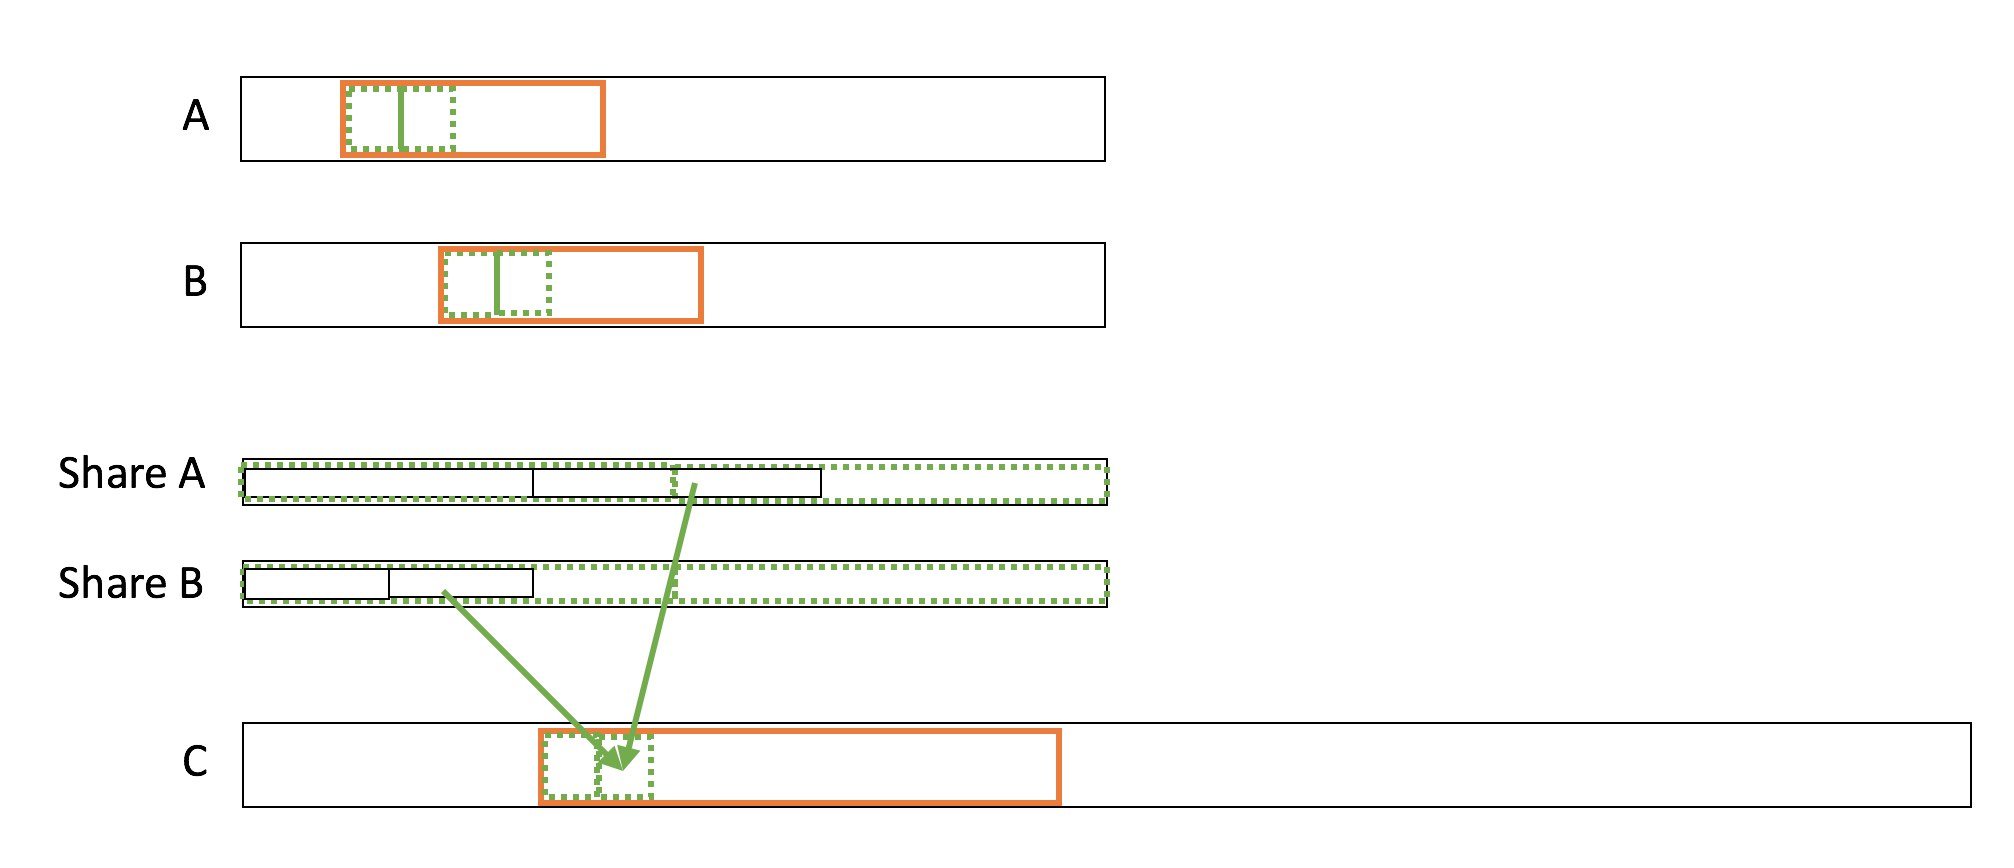
\includegraphics[width=\textwidth]{double2.png}
    \end{center}
    \caption{{\label{fig:double2}} Second Iteration of Double Buffer Parallel Merge}
    \end{figure}

    If there are less than $x$ elements in either shared array A or shared array B, 
    we will load another $x$ elements the into shared memory. Figure \ref{fig:double3} 
    shows an example of the third iteration of double buffer parallel 
    merge. In the third iteration, there are enough data in the shared array B. However,
    there are not enough (less than $x$) data in shared array A. So we load $x$ elements 
    from the global memory to shared memory (marked by the red box). Data in shared memory 
    will wrap around.  

    \begin{figure}[!h]
    \begin{center}
    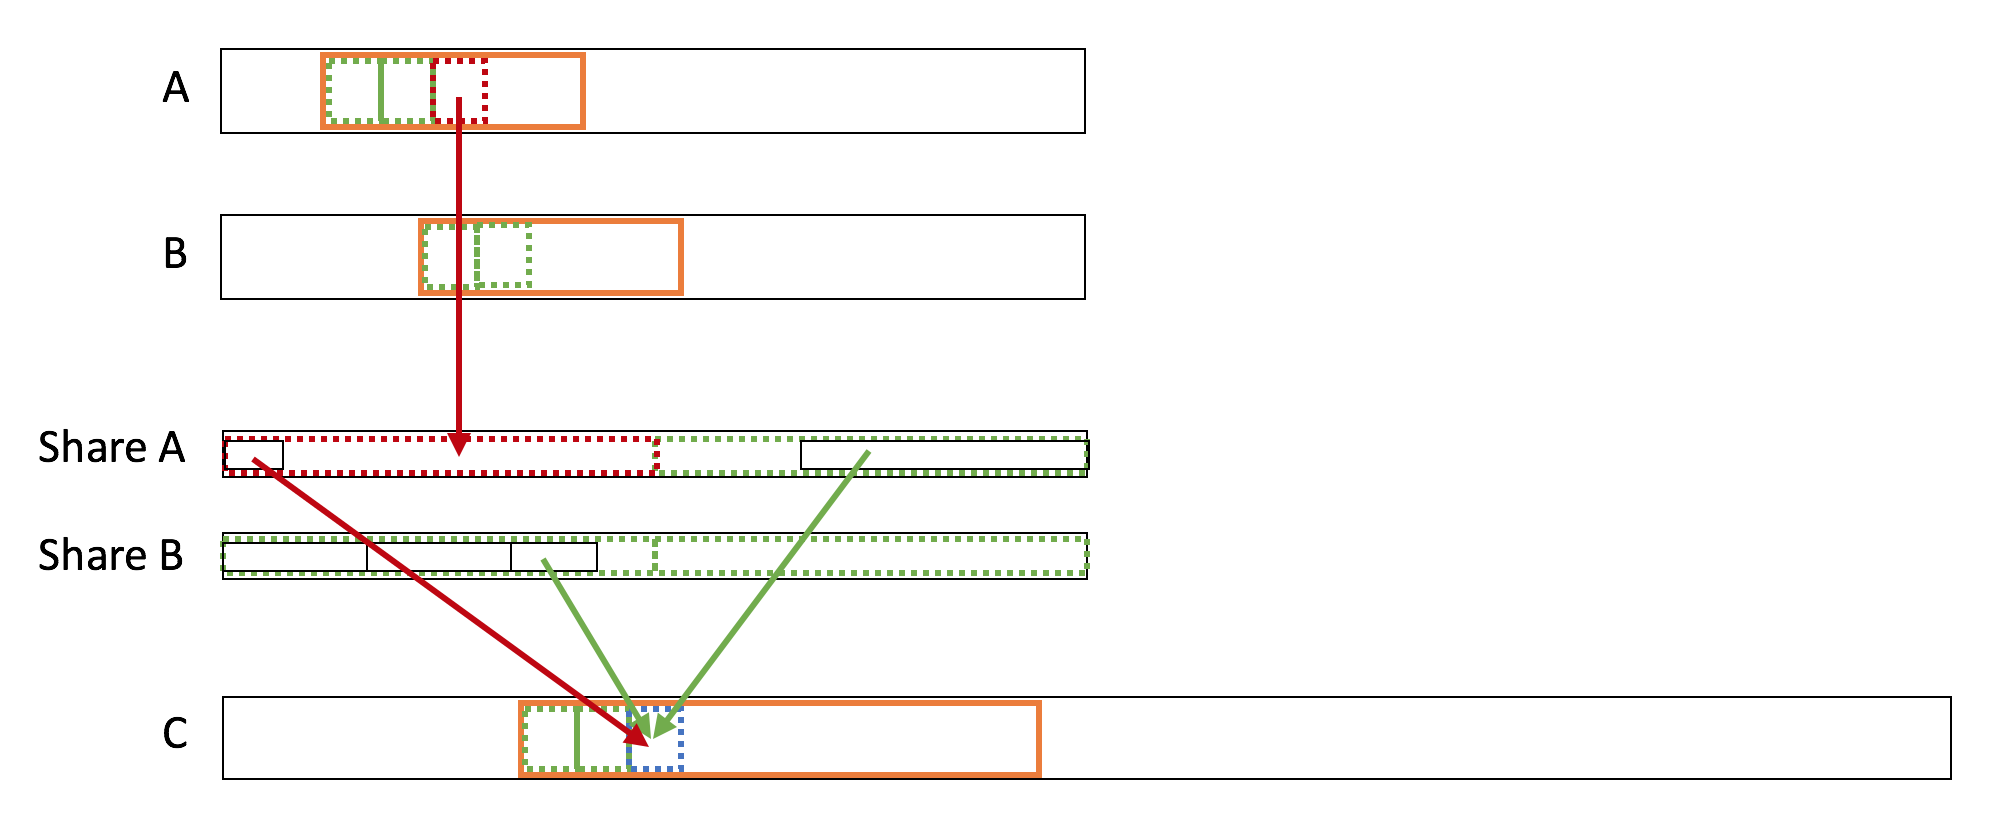
\includegraphics[width=\textwidth]{double3.png}
    \end{center}
    \caption{{\label{fig:double3}} Third Iteration of Double Buffer Parallel Merge}
    \end{figure}
 
    Then we run the co-rank function in thread level. The co-rank function is run on 
    shared memory. Each thread calculates the thread index and total number of threads 
    in the block using $t\_id = threadIdx.x$ and $r\_num = blockDim.x$ respectively. 
    Based on $t\_id$ and $t\_num$, each thread calculates the output range 
    that thread is going to produce, and uses the output range as the input to the co-rank function 
    to identify the corresponding input ranges.  
    Then each thread can start its work independently and call the sequential merge function to do 
    the merge in parallel on the input we load to shared memory and write the output to device 
    global memory.

    The loop runs until we have merged all the data that block is going to produce (filling 
    the entire solid orange box).   

    Notice that the memory access pattern of double buffer parallel merge is coalesced. 
    In double buffer parallel merge, we utilize all the 
    data we load into shared memory, while in single buffer parallel merge, we waste half of 
    the data we load into shared memory. We expect that double buffer parallel merge will 
    outperform single buffer parallel merge. However, in experiments, we observed that double 
    buffer used more registers (39) than single buffer parallel merge (31), and caused the occupancy 
    to drop. As a result, the double buffer parallel merge is not as fast as single buffer parallel
    merge. 

    The performance of double buffer parallel merge is evaluated in Figure \ref{fig:double_evaluation}.

    \begin{figure}[!h]
    \begin{center}
    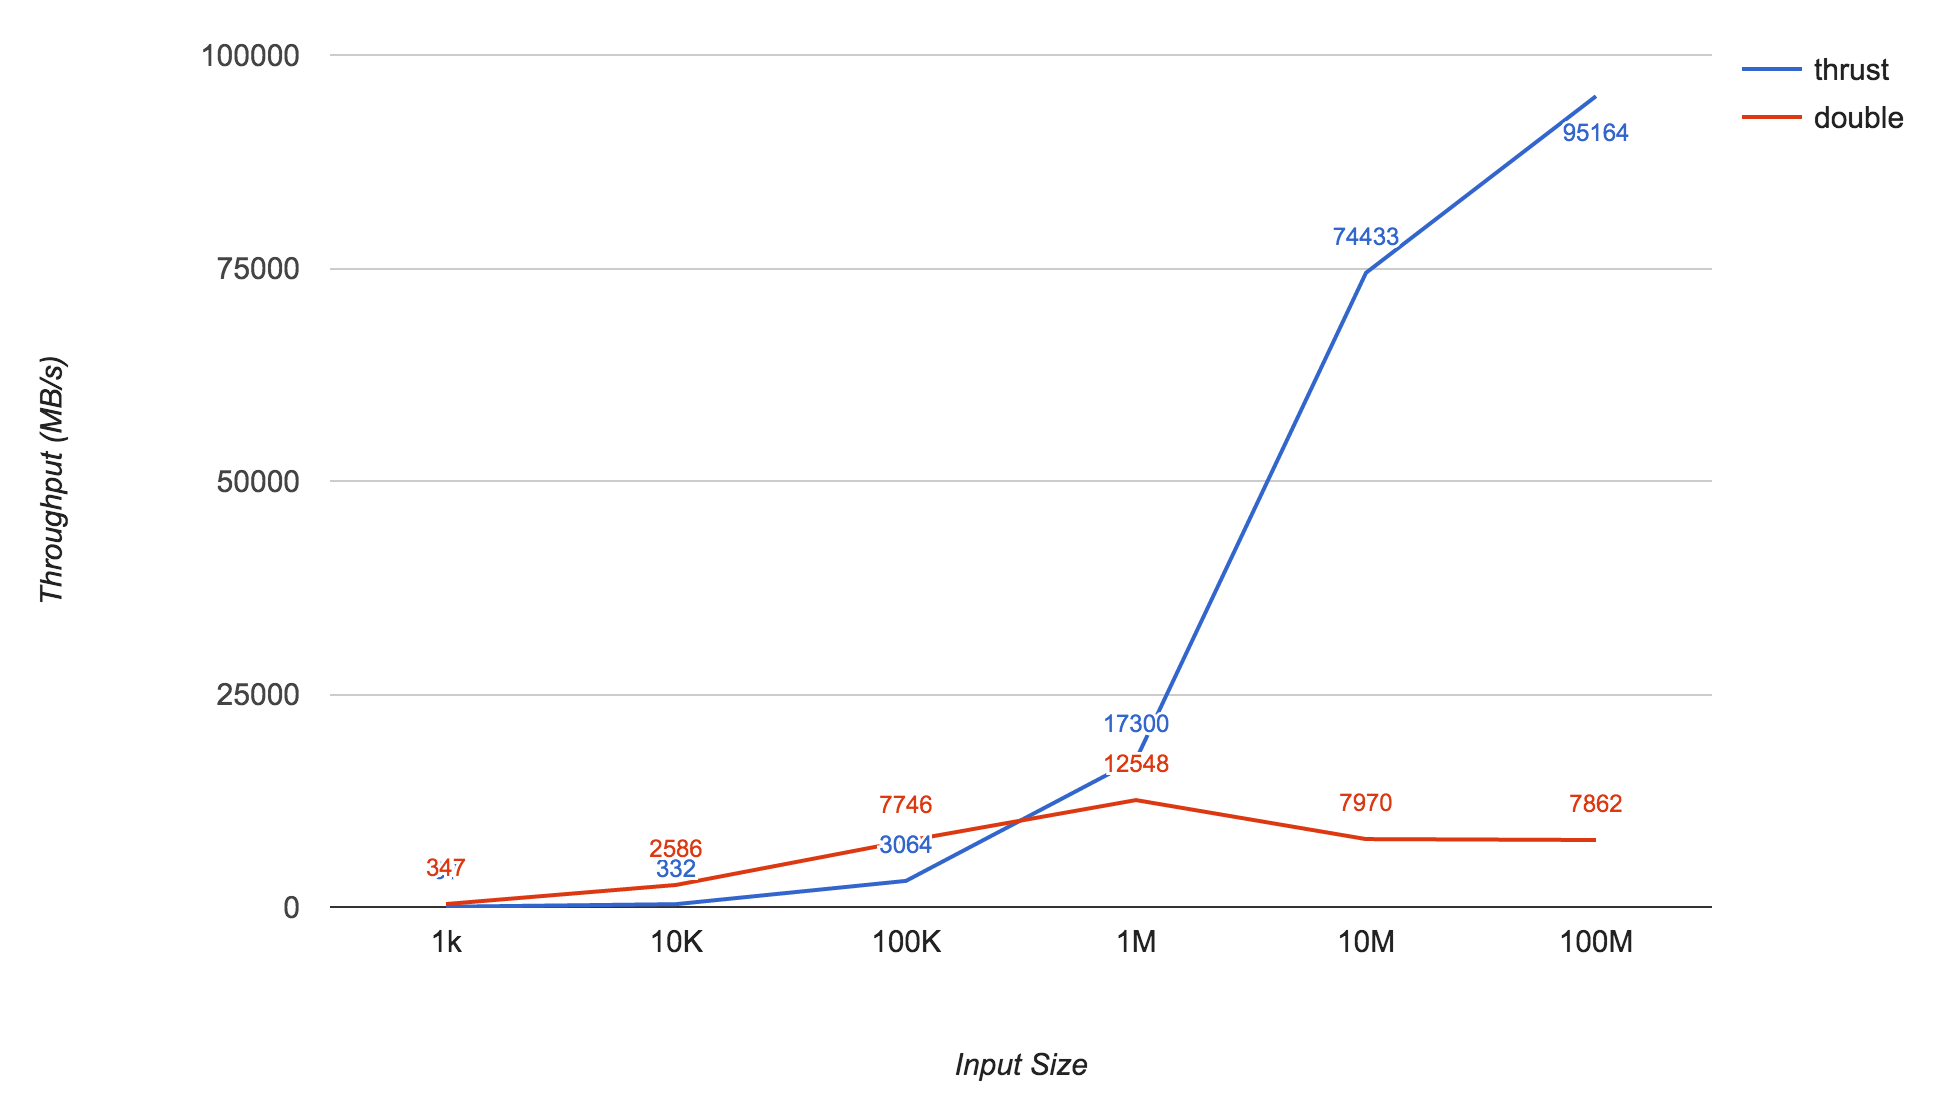
\includegraphics[width=\textwidth]{double_evaluation.png}
    \end{center}
    \caption{{\label{fig:double_evaluation}} Performance of Double Buffer Parallel Merge on Titan-Z}
    \end{figure}

%%%%%%%%%%%%%%%%%%%%%%%%%%%%%%%%%%%%%%%%%%%%%%%%%%%%%%%%%%%%%%%%
%   
%   Further Optimizations
%

    \section{Further Optimizations}\label{sect:opt}
        \subsection{Reduce Number of Calls to Co-rank Function}\label{sect:opt:co-rank}
        In all the GPU parallel merge implementations above, each thread needs to call the co-rank 
        function twice: once for the start point of the output range, and once for the end point 
        of the output range. Figure \ref{fig:reduce-0} gives an example. In this example, there 
        are $8$ threads. We mark the call to co-rank function using ``$*$". 
        Each thread will call co-rank twice to calculate $j\_start$ and $j\_end$.
        Therefore, the total number of calls to co-rank function is $16$.  

        \begin{figure}[!h]
        \begin{center}
        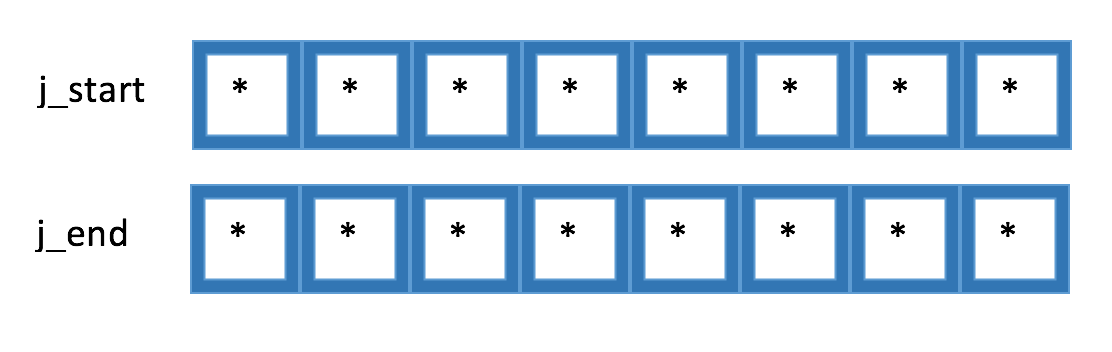
\includegraphics[width=\textwidth]{reduce-0.png}
        \end{center}
        \caption{{\label{fig:reduce-0}} Number of Calls to Co-rank Function}
        \end{figure}

        One observation we have is that the start point of thread $r$ is the same as 
        the end point of thread $r-1$. In the example we provide in figure \ref{fig:overall}, 
        the start point of $p1$ is $8$ and the end point of $p0$ is also $8$. 
        For this reason, we could reduce the number of calls to co-rank function. 
        We first let all the threads calculate the co-rank for the end point, 
        as shown in figure \ref{fig:reduce-1}.
        Instead of using co-rank function again to calculate the co-rank for starting point,
        we store the result($j\_end$) in an array in shared memory.  
        Then after a synchronization, we read the co-rank of start point of thread $r$
        from the result of thread $r-1$. If thread index is $0$, we will set the co-rank to $0$ 
        instead of reading from thread $-1$. Now we only need to call co-rank function for
        $8$ times (as marked by ``$*$" in figure \ref{fig:reduce-1}) and reduce the number of calls by half.     

        \begin{figure}[!h]
        \begin{center}
        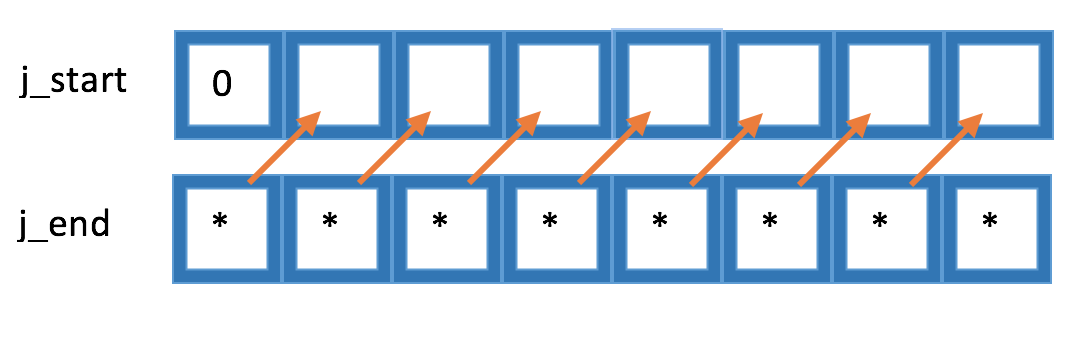
\includegraphics[width=\textwidth]{reduce-1.png}
        \end{center}
        \caption{{\label{fig:reduce-1}} Number of Calls to Co-rank Function after Optimization}
        \end{figure}


        \subsection{Change Code Divergence to Memory Divergence}\label{set:opt:div}
        Code divergence also hurts the performance of GPU application. When the threads in the 
        same warp take different branches for an $if-else$ statement, code divergence will occur.
        The hardware needs to execute the $if$ part and $else$ part sequentially. This will 
        hurt the overall performance. As a result, it is desirable 
        to write code with a minimum amount of code divergence to achieve high performance.
        In parallel merge, we are concerned about two functions: merge and co-rank.   
        \begin{itemize}
            \item Merge\\ 
                  Listing \ref{list:merge_origin} shows the original sequential merge code. 
                  It uses a while
                  loop to do the merge. It first merges A and B to C, and then copies the 
                  remaining A 
                  or B to C. We can see that the original merge has code divergence due to 
                  \textbf{if} and \textbf{else} statements inside the while loop. 
                  To remove the code divergence, we use \textbf{selection} to replace the 
                  \textbf{if} and \textbf{else} statements.
                  Listing  \ref{list:merge_nodiv} shows the sequential merge code after removing 
                  code divergence. After this optimization, we effectively replace all the code
                  divergence with memory divergence. 
            \item Co-rank\\
                  Listing \ref{list:corank_origin} shows the original code for co-rank function. 
                  The code divergence also comes from the \textbf{if} and \textbf{else} statements. We replace
                  the \textbf{if} and \textbf{else} statements by \textbf{selection}. The resulting code is 
                  shown in Listing \ref{list:corank_nodiv}.
        \end{itemize}

        \begin{minipage}{\linewidth}
        \begin{singlespace}
        \begin{lstlisting} [caption = {Merge Remove Code Divergence}, captionpos=b, label = {list:merge_nodiv}]
void merge(int *A, int m, int*B, int n, int*C) 
{
  int count = m+n;
  int ai = 0, bi=0;
  for(int i=0; i< count; ++i)
  {
    bool p;
    bool c1 = (bi >= n);
    bool c2 = (ai >= m);
    p = c1 ? true : c2 ? false : A[ai]>B[bi] ? false : true; 
    C[i] = p ? A[ai++] : B[bi++];
  }
}
        \end{lstlisting}
        \end{singlespace}
        \end{minipage}

        \begin{minipage}{\linewidth}
        \begin{singlespace}
        \begin{lstlisting} [caption = {Co-rank Remove Code Divergence}, captionpos=b, label = {list:corank_nodiv}]
int co_rank_j(int i, int* A, int m, int* B, int n)
{
    int j = i<m ? i : m;                //j = min(i,m)
    int k = i - j;
    int j_low = 0>(i-n) ? 0 : i-n;      //j_low = max(0, i-n) 
    int k_low;
    int delta;

    while(1)
    {
        bool cond_1 = j > 0 && k <n && A[j-1] > B[k];
        bool cond_2 = k > 0 && j <m && B[k-1] >= A[j];
        
        delta = cond_1 ? ((j-j_low-1)>>1) + 1 : 
                cond_2 ? ((k-k_low-1)>>1) + 1 : delta;
        k_low = cond_1 ? k : k_low;
        j_low = cond_2 ? j : j_low;
        j     = cond_1 ? j - delta : cond_2 ? j+delta : j;
        k     = cond_1 ? k + delta : cond_2 ? k-delta : k;
        if(!cond_1 && !cond_2)
            break;
    }
    return j;
}
        \end{lstlisting}
        \end{singlespace}
        \end{minipage}

        After removing code divergence, we see some speedup.

        Here is a figure.

    \section{Tuning Parameters}\label{sect:tuning}
    We set the number of blocks, the block dimension, and shared memory size as our tuning
    parameters.
    \begin{itemize}
    \item \textbf{number of blocks:} When we change the number of blocks, we are also changing
           the amount of work for each block. When we increase the number of blocks, we create 
           more parallelism that could be scheduled on different SM. Meanwhile, the amount of 
           work for each block is decreasing. We want the amount of work for each block to be
           large enough to amortize the block launch overhead. We choose the number of blocks 
           from 1, 4, 16, 64, 256, and 512.
    \item \textbf{block dimension:} Block dimension determines the number of threads in the 
           thread block. We choose the block dimension from 128, 256, and 512.
    \item \textbf{shared memory size:} Shared memory size can affect the number of blocks that
          can run simultaneously on the SM. We choose from 1024B, 2048B and 2560B. 
    \end{itemize}

    We enumerate all the combinations of tuning parameters, record their running time, and 
    choose the one that has the best performance.



\chapter{Evaluation}\label{chap:evaluation}
We put the performance of all the parallel merge implementations 
on Titan-Z in Chapter \ref{chap:implementation} in Figure \ref{fig:titan-z}.
\begin{figure}[!bh]
\begin{center}
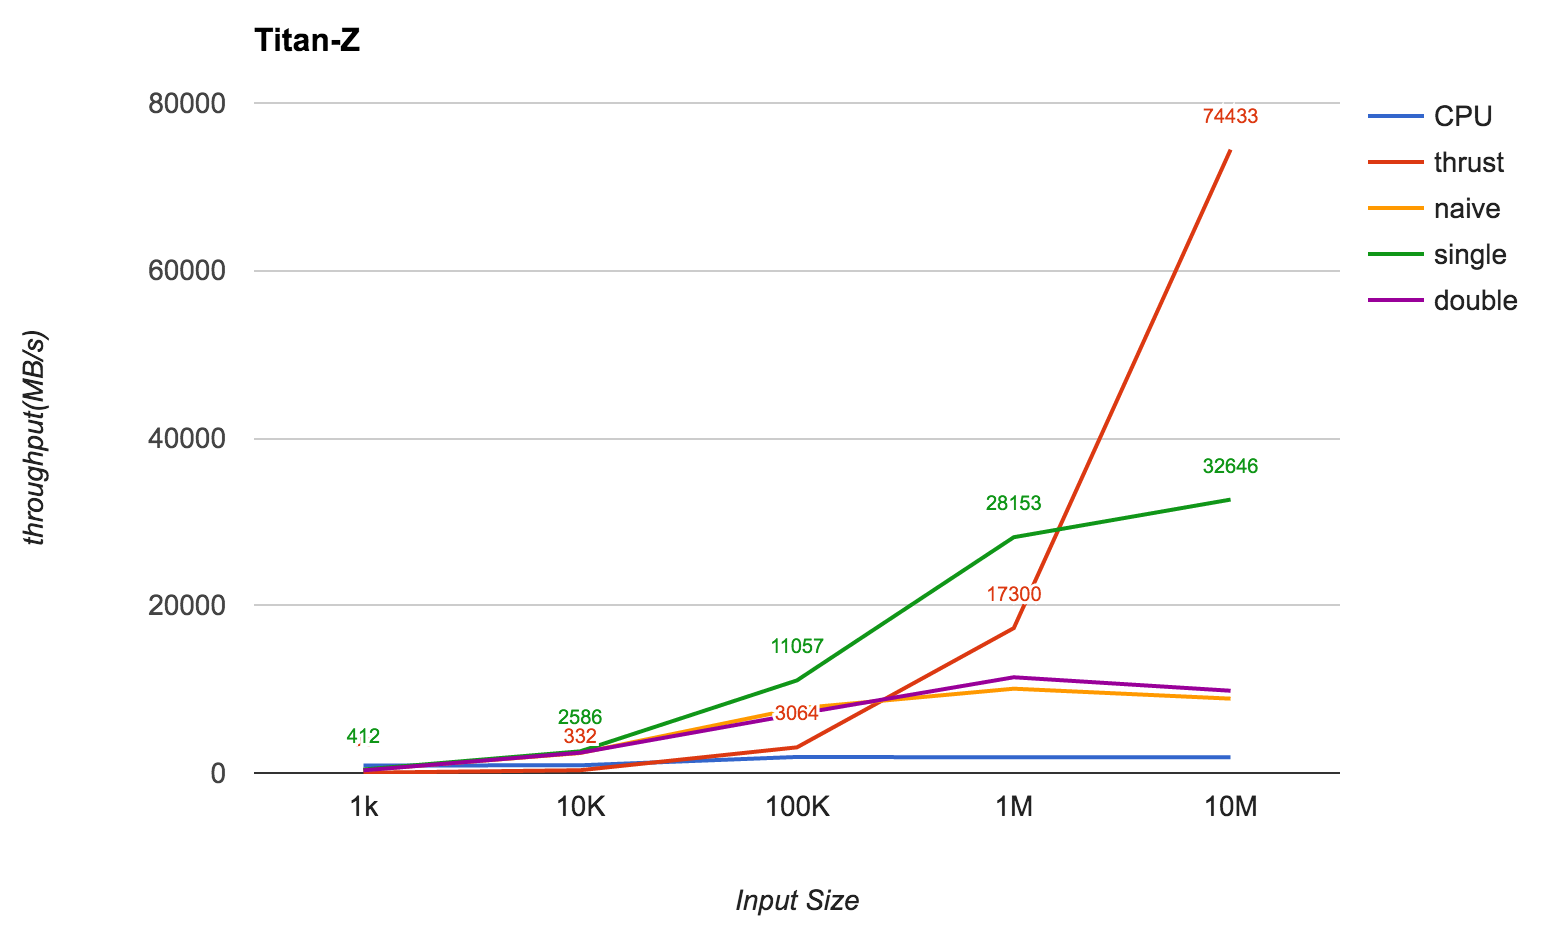
\includegraphics[width=\textwidth]{titan-z.png}
\end{center}
\caption{{\label{fig:titan-z}} Performance on Titan-Z}
\end{figure}

Among the three implementations we have, single buffer parallel merge has the 
best performance. Compared to thrust merge implementation, single buffer 
parallel merge can achieve up to 3x speedup for input size between 10k to 1M.

We also test the portability of our implementations on an Nvidia GTX980 GPU (Maxwell 
Architecture). Figure \ref{fig:maxwell} shows the performance.
\begin{figure}[!bh]
\begin{center}
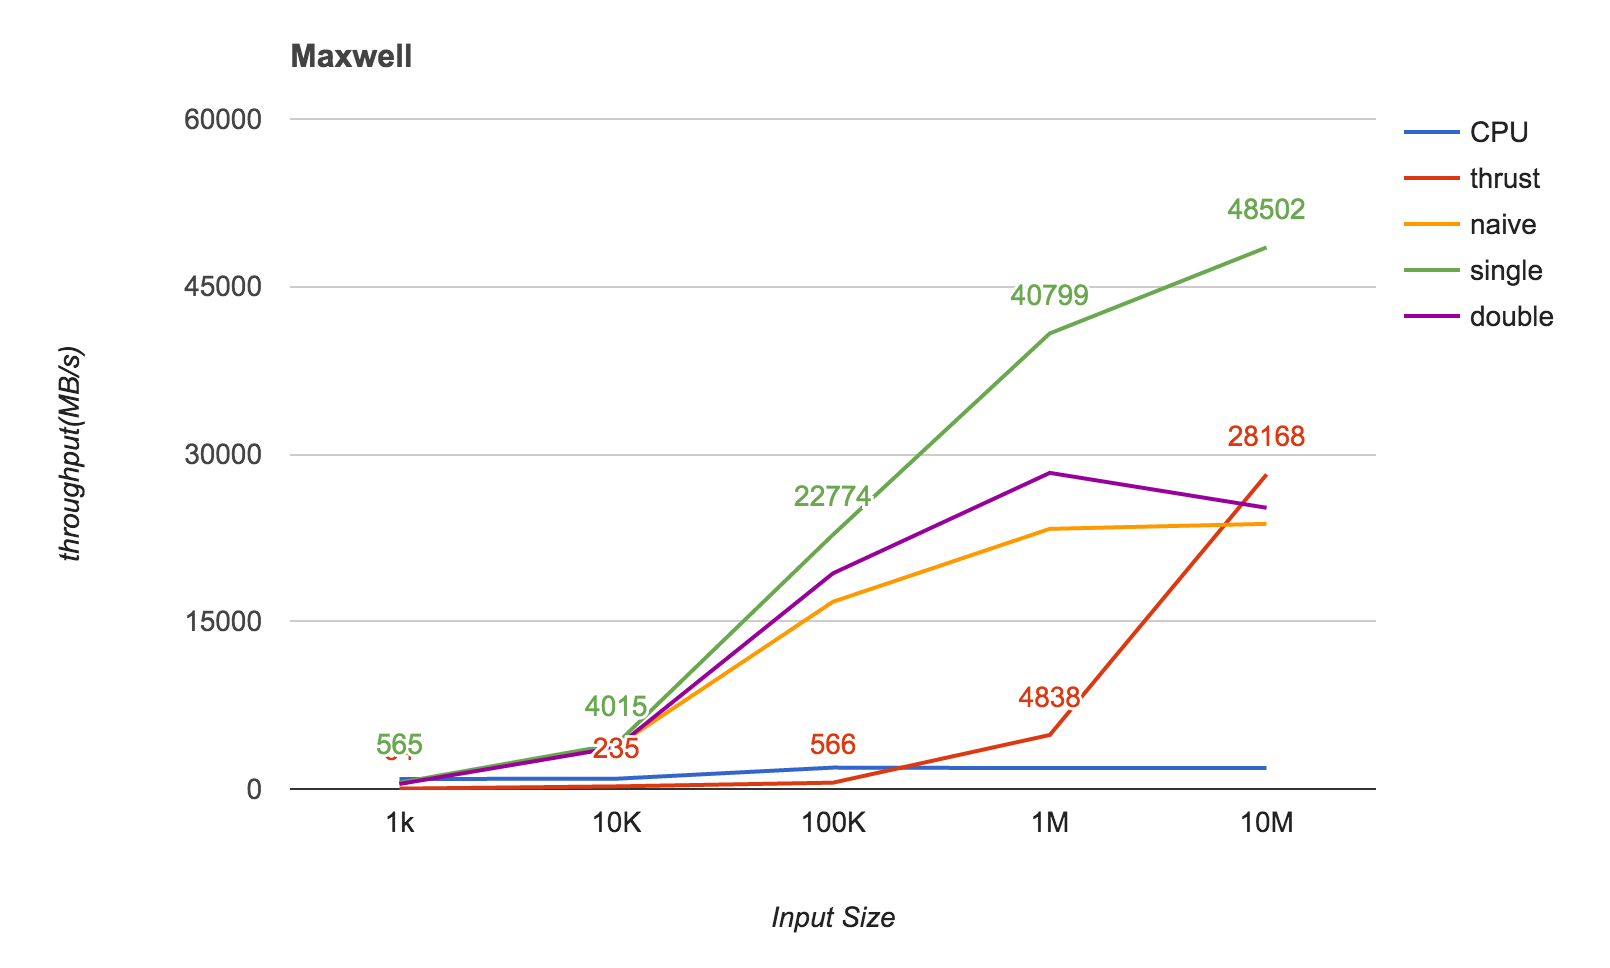
\includegraphics[width=\textwidth]{maxwell.png}
\end{center}
\caption{{\label{fig:maxwell}} Performance on GTX980}
\end{figure}

Single buffer parallel merge outperforms the other two implementations as well.
Compared to thrust merge, single buffer parallel merge can achieve up to 20x 
speedup. The reason is that thrust merge is not specifically optimized for 
Maxwell Architecture and therefore its performance is far from optimal on this 
architecture. 

\chapter{Conclusion}\label{chap:conclusion}
In this thesis, we implemented three versions of parallel merge algorithm on GPU: 
naive parallel merge, single buffer parallel merge and double buffer parallel merge.

We evaluated their performance on different GPUs. Among the three versions, single 
buffer parallel merge had the best performance. Compared to sequential merge,
single buffer parallel merge achieved 10x speedup. Compared to thrust merge 
implementation, single buffer parallel merge achieved at most 20x speedup 
for certain GPU architecture.


%\include{exper}
%\include{concl}


%%%%%%%%%%%%%%%%%%%%%%%%%%%%%%%%%%%%%%%%%%%%%%%%%%%%%%%%%%%%%%%%%%%%%%%%%%%%%%%
% APPENDIX
%
\appendix
%\include{apx}

\backmatter

%%%%%%%%%%%%%%%%%%%%%%%%%%%%%%%%%%%%%%%%%%%%%%%%%%%%%%%%%%%%%%%%%%%%%%%%%%%%%%%
% BIBLIOGRAPHY
%
\bibliographystyle{IEEE_ECE}
% Put references in BibTeX format in thesisrefs.bib.
\bibliography{thesisrefs}


%%%%%%%%%%%%%%%%%%%%%%%%%%%%%%%%%%%%%%%%%%%%%%%%%%%%%%%%%%%%%%%%%%%%%%%%%%%%%%%
% AUTHOR'S BIOGRAPHY
% As of 10/03/2011, Author's Biography or Vita no longer accepted by Grad College

\end{document}
\endinput
